% =============================================================================
% Artigo da Iniciação Científica — Lucas Teixeira Correia
% Plano de trabalho: Otimização do dimensionamento e posicionamento de fundações
% superficiais de edifícios considerando conceitos de empacotamento e mecânica
% das estruturas.
% Orientadora: Profa. Maria José Pereira Dantas (PUC Goiás)
%
% Recorte do artigo:
%   Surrogate-assisted optimization (EGO + GPR + AG) para o dimensionamento
%   automatizado de sapatas isoladas, com abertura metodológica para a etapa
%   subsequente de empacotamento (layout) das fundações.
%
% Status: versão experimental consolidada; limitações declaradas no texto.
% Compilação: pdflatex main && bibtex main && pdflatex main && pdflatex main
% =============================================================================
\documentclass[10pt,a4paper,twocolumn]{article}

% --- Codificação e idioma -----------------------------------------------------
\usepackage[utf8]{inputenc}
\usepackage[T1]{fontenc}
\usepackage[english,brazilian]{babel}
\usepackage{lmodern}
\usepackage{microtype}

% --- Estrutura e formatação ---------------------------------------------------
\usepackage[a4paper,margin=2.0cm,columnsep=0.8cm]{geometry}
\usepackage{setspace}
\singlespacing
\usepackage{indentfirst}
\usepackage{balance}   % equaliza as colunas da última página
\usepackage{titlesec}
\titleformat{\section}{\large\bfseries}{\thesection}{1em}{}
\titleformat{\subsection}{\normalsize\bfseries}{\thesubsection}{1em}{}
\titleformat{\subsubsection}{\normalsize\itshape}{\thesubsubsection}{1em}{}

% --- Matemática e ciência -----------------------------------------------------
\usepackage{amsmath,amssymb,amsthm,bm}
\usepackage{mathtools}
\usepackage{siunitx}
\sisetup{output-decimal-marker={,},group-separator={\,},per-mode=symbol,
         range-phrase={ a },range-units=single}

% --- Figuras e tabelas --------------------------------------------------------
\usepackage{graphicx}
\graphicspath{{figuras/}}
\usepackage{booktabs}
\usepackage{caption}
\captionsetup{font=small,labelfont=bf}
\usepackage{subcaption}
\usepackage{float}

% --- Algoritmos e código ------------------------------------------------------
\usepackage[ruled,vlined,linesnumbered]{algorithm2e}
\usepackage{listings}
\lstset{basicstyle=\ttfamily\small,frame=single,breaklines=true}

% --- Referências cruzadas e citações -----------------------------------------
\usepackage[hidelinks]{hyperref}
\usepackage{cleveref}
\usepackage{url}

% --- Citações ABNT (autor-data) ----------------------------------------------
\usepackage[alf,abnt-emphasize=bf,abnt-thesis-year=both,abnt-etal-list=0]{abntex2cite}

% --- Macros do projeto --------------------------------------------------------
\usepackage{xspace}
\newcommand{\fundaai}{\textsc{FundaAI}\xspace}
\newcommand{\citepabnt}[1]{(\citeauthoronline{#1}, \citeyear{#1})}
\newcommand{\citepabnttwo}[2]{(\citeauthoronline{#1}, \citeyear{#1}; \citeauthoronline{#2}, \citeyear{#2})}
\newcommand{\citepabntthree}[3]{(\citeauthoronline{#1}, \citeyear{#1}; \citeauthoronline{#2}, \citeyear{#2}; \citeauthoronline{#3}, \citeyear{#3})}
\newcommand{\citepabntfour}[4]{(\citeauthoronline{#1}, \citeyear{#1}; \citeauthoronline{#2}, \citeyear{#2}; \citeauthoronline{#3}, \citeyear{#3}; \citeauthoronline{#4}, \citeyear{#4})}

% =============================================================================
\begin{document}

% --- Cabeçalho e resumos em largura total (duas colunas começam depois) -------
% O grupo {...} protege os colchetes internos (ex.: \item[]) do argumento
% opcional de \twocolumn.
\twocolumn[{
\begin{@twocolumnfalse}
\begin{center}
    {\LARGE \bfseries Otimização computacional do pré-dimensionamento geométrico de sapatas isoladas: uma abordagem com modelo substituto e metaheurística \par}

    \vspace{0.4cm}
    {\large \textit{Computational design optimization of isolated shallow foundations using surrogate modelling and metaheuristics}\par}

    \vspace{0.5cm}
    {\normalsize Lucas Teixeira Correia\textsuperscript{1}\par}
    {\small \textsuperscript{1}Pontifícia Universidade Católica de Goiás, Escola de Engenharia, Goiânia, GO, Brasil\par}
    {\small Grupo de Pesquisa: \textit{Identification, Modeling and Artificial Intelligence for Systems Optimization}\par}
\end{center}

\vspace{0.3cm}

% --- Resumo ------------------------------------------------------------------
\begin{list}{}{\setlength{\leftmargin}{1.2em}\setlength{\rightmargin}{1.2em}}
\item[]\small
\noindent \textbf{Resumo.}
Este artigo apresenta uma abordagem computacional para o pré-dimensionamento geométrico de sapatas isoladas, formulada como minimização do volume de concreto com restrições de tensão admissível do solo, geometria mínima, punção e não sobreposição. A solução combina \textit{Efficient Global Optimization} (EGO), Regressão por Processos Gaussianos (GPR) e Algoritmo Genético (AG) para orientar avaliações sequenciais da função pseudo-objetivo, além de uma variante de otimização bayesiana com restrições que modela volume e viabilidade separadamente. O protocolo experimental considera três casos de estudo, 30 repetições pareadas, orçamento de 150 avaliações reais e comparação com AG, PSO, GWO e busca aleatória, incluindo um cenário de orçamento estendido para as buscas diretas. Com 150 avaliações, a variante com restrições explícitas apresentou as menores médias de $\Theta$ nos três casos e reduziu a mediana em até $71{,}4\,\%$ frente à busca aleatória, mas com menor factibilidade estrita nos dois casos menores. Com $3\,000$ avaliações, as buscas diretas superaram as referências assistidas por modelo substituto em menor tempo, pois a avaliação atual tem baixo custo computacional. Uma auditoria por decomposição mostrou ganhos de apenas $<0{,}01\,\%$, $0{,}77\,\%$ e $2{,}08\,\%$ sobre o melhor volume factível global, confirmando que os casos são quase separáveis. O estudo de penalidade indicou que fatores elevados preservam o $R^2$ global, mas degradam o erro na região factível; a escolha do \textit{kernel} foi secundária. Os resultados delimitam a abordagem como pré-dimensionamento experimental e motivam a etapa futura de posicionamento com restrições de empacotamento.

\noindent \textbf{Palavras-chave:} Otimização global. Fundações superficiais. Modelo substituto. Processos gaussianos. Algoritmo genético. Empacotamento.

\vspace{0.3cm}

\begin{otherlanguage}{english}
\noindent \textbf{Abstract.}
This paper presents a computational approach for the geometric pre-design of isolated footings, formulated as concrete-volume minimisation with constraints on allowable soil pressure, minimum geometry, punching shear and overlap. The solution combines \textit{Efficient Global Optimization} (EGO), Gaussian Process Regression (GPR) and a Genetic Algorithm (GA) to guide sequential evaluations of the pseudo-objective function, and also evaluates a constrained Bayesian optimisation variant that models volume and feasibility separately. The experimental protocol includes three case studies, 30 paired repetitions, a budget of 150 real evaluations and comparisons with GA, PSO, GWO and random search, plus an extended-budget scenario for direct searches. With 150 evaluations, the constraint-aware variant achieved the lowest mean $\Theta$ in all three cases and reduced the median by up to 71.4\% relative to random search, but with lower strict feasibility in the two smaller cases. With 3,000 evaluations, direct searches outperformed the surrogate-assisted references in less wall-clock time because the current objective evaluation is inexpensive. A decomposition audit found gains of only $<0.01\%$, $0.77\%$ and $2.08\%$ over the best global feasible volume, confirming that the current cases are nearly separable. The penalty study showed that large penalty factors preserve global $R^2$ while degrading feasible-region error; kernel choice was secondary. The results position the approach as an experimental pre-design method and motivate the next stage on foundation positioning with packing constraints.

\noindent \textbf{Keywords:} Global optimisation. Shallow foundations. Surrogate model. Gaussian processes. Genetic algorithm. Packing.
\end{otherlanguage}
\end{list}

\vspace{0.5cm}
\end{@twocolumnfalse}
}]

% --- Seções (modulares) ------------------------------------------------------
% =============================================================================
% Seção 1 — Introdução
% =============================================================================
\section{Introdução}
\label{sec:introducao}

As fundações compõem o subsistema estrutural responsável por transferir as ações da superestrutura ao maciço de solo de apoio, exercendo papel determinante na estabilidade global, na limitação de recalques diferenciais e na viabilidade econômica das edificações \citepabnt{abnt6122}. Em especial, as fundações superficiais do tipo sapata isolada apresentam ampla aplicação em edificações de pequeno e médio porte, em razão da simplicidade construtiva e do baixo custo associado \citepabnttwo{wang2008economic}{waheed2022practical}.

A despeito de sua frequência em obras correntes, o dimensionamento dessas fundações é, na prática profissional, frequentemente conduzido por procedimentos iterativos de tentativa e verificação, nos quais o engenheiro arbitra dimensões e verifica, sucessivamente, o atendimento a critérios de projeto associados à tensão admissível do solo, à punção e à compatibilidade geométrica entre o pilar e a sapata \citepabntthree{wang2008economic}{khajehzadeh2012gsa}{gandomi2018construction}. Esse fluxo de trabalho depende da experiência do projetista e pode produzir soluções viáveis, porém conservadoras, com consumo de concreto superior ao obtido por formulações de otimização econômica \citepabnttwo{waheed2022practical}{waheed2025optimization}.

A elevada pegada de carbono associada à produção do cimento e à execução das fundações reforça a relevância da racionalização do volume de concreto empregado. Ferramentas computacionais que automatizem a busca por soluções de menor consumo material podem, portanto, contribuir para a sustentabilidade das obras de engenharia civil, desde que preservados os critérios de segurança e desempenho \citepabnt{waheed2025optimization}. Nesse contexto, métodos de otimização baseados em metaheurísticas e em técnicas de aprendizado de máquina vêm sendo aplicados a problemas de projeto estrutural e geotécnico, dada a sua capacidade de explorar espaços de busca não convexos, de elevada dimensionalidade e com restrições heterogêneas \citepabntfour{gomes2018probabilistic}{morales2020balance}{abualigah2021arithmetic}{kashani2020optimum}.

Este estudo se insere nesse cenário e investiga a seguinte pergunta de pesquisa: \textit{é possível desenvolver uma abordagem computacional que realize o pré-dimensionamento geométrico e, em etapa posterior, o posicionamento otimizado de fundações superficiais, integrando verificações estruturais e geotécnicas em um único ambiente, de forma a reduzir o consumo de concreto e o esforço manual do projetista?}

Como recorte específico deste artigo, apresentam-se os resultados relativos à \textit{primeira} frente da pesquisa: o pré-dimensionamento geométrico otimizado das sapatas isoladas, considerando posições de pilares fornecidas pelo projeto estrutural e um conjunto limitado de verificações de tensão no solo, geometria e punção. A abordagem adotada é a otimização global assistida por modelo substituto, mais especificamente o método \textit{Efficient Global Optimization} (EGO) proposto por \citeonline{jones1998efficient}, no qual um Processo Gaussiano (GPR) atua como modelo substituto da função objetivo \citepabntthree{williams1995gaussian}{schulz2018tutorial}{shahriari2016review}, e um Algoritmo Genético (AG) é empregado como otimizador interno na maximização da função de aquisição \textit{Expected Improvement} (EI). A frente complementar -- a incorporação do problema de empacotamento ao posicionamento conjunto das fundações -- é objeto da próxima etapa do plano de trabalho e não é tratada de forma exaustiva neste manuscrito.

Como a função pseudo-objetivo desta etapa tem baixo custo computacional na implementação vetorizada atual, a adequação da arquitetura assistida por modelo substituto não é assumida: ela é avaliada empiricamente neste artigo sob dois regimes de orçamento — eficiência amostral com número igual de avaliações reais e tempo de parede com orçamento estendido para as buscas diretas — e complementada por uma auditoria de decomposição por sapata. Com isso, delimita-se o domínio em que o EGO é a escolha vantajosa, o domínio em que buscas diretas são suficientes e o limite metodológico imposto pela quase separabilidade dos casos atuais.

\subsection{Objetivos}
\label{sec:objetivos}

\paragraph{Objetivo geral.} Apresentar e discutir, do ponto de vista metodológico e experimental, uma abordagem computacional assistida por modelo substituto para o pré-dimensionamento geométrico de sapatas isoladas, integrando verificações parciais da mecânica das estruturas e da geotecnia, e implementada em uma plataforma computacional (\fundaai{}) construída em Python.

\paragraph{Objetivos específicos.}
\begin{enumerate}
    \item Revisar criticamente o estado da arte recente em otimização aplicada ao projeto de fundações superficiais, com ênfase em metaheurísticas e em métodos baseados em modelos substitutos.
    \item Formular o problema de pré-dimensionamento geométrico de sapatas isoladas como uma otimização mono-objetivo penalizada, combinando critérios inspirados na NBR~6118 \citepabnt{abnt6118} e na NBR~6122 \citepabnt{abnt6122}, correlações empíricas e hipóteses explícitas de pré-dimensionamento.
    \item Apresentar os fundamentos teóricos do método EGO e do GPR e discutir criticamente a escolha dessa arquitetura híbrida em uma formulação que, nesta etapa, possui avaliação direta de baixo custo, mas prepara o método para extensões com maior custo de avaliação e restrições mais complexas.
    \item Reportar, sob protocolo experimental fechado (sementes registradas, orçamento de avaliações equalizado e teste estatístico pareado), o efeito do fator de penalidade e da escolha do \textit{kernel} sobre a qualidade preditiva do modelo substituto, a comparação da arquitetura proposta com Algoritmo Genético, PSO, GWO, busca aleatória e uma variante com tratamento explícito de restrições (\textit{Constrained Bayesian Optimization}) em dois regimes de orçamento, e uma auditoria de quase separabilidade por decomposição de sapatas.
    \item Discutir as limitações da abordagem atual e situar, como trabalho subsequente, a incorporação explícita do problema de \textit{empacotamento} para o posicionamento conjunto e o dimensionamento das fundações.
\end{enumerate}

\subsection{Contribuição e estrutura do artigo}
\label{sec:contribuicao}

A principal contribuição deste artigo é apresentar, em formato consolidado, uma arquitetura EGO--GPR--AG aplicada à minimização do volume de concreto de sapatas isoladas e discutir as escolhas de modelagem que afetam a qualidade preditiva do modelo substituto -- em particular, o fator de penalidade aplicado às restrições e a função de covariância do GPR --, quantificando ainda, sob protocolo controlado, quando o tratamento explícito das restrições por otimização bayesiana com restrições supera a penalização direta. O artigo também inclui uma linha de base por decomposição para explicitar o quanto os casos atuais são quase separáveis. Adicionalmente, o trabalho documenta a implementação de uma plataforma computacional (\fundaai{}) que integra leitura de dados de projeto, parametrização do otimizador, execução do método e visualização dos arranjos resultantes, com todos os resultados regeneráveis por \textit{scripts} determinísticos a partir de artefatos persistidos.

O restante do artigo está organizado da seguinte forma. A Seção~\ref{sec:estado_da_arte} apresenta o estado da arte sobre otimização aplicada ao dimensionamento de fundações superficiais e o panorama metodológico das técnicas baseadas em modelos substitutos. A Seção~\ref{sec:fundamentacao} introduz a fundamentação teórica do EGO, do GPR e da função de aquisição EI. A Seção~\ref{sec:metodologia} formaliza o problema de otimização e descreve a arquitetura proposta. A Seção~\ref{sec:implementacao} detalha a implementação computacional da ferramenta \fundaai{}. A Seção~\ref{sec:resultados} reporta os resultados do protocolo experimental. A Seção~\ref{sec:discussao} discute esses resultados de forma integrada com as referências da literatura. Por fim, a Seção~\ref{sec:conclusoes} sintetiza as conclusões e aponta os trabalhos futuros, com destaque para a frente de empacotamento.

% =============================================================================
% Seção 2 — Estado da arte
% =============================================================================
\section{Estado da arte}
\label{sec:estado_da_arte}

\subsection{Otimização aplicada ao projeto de fundações superficiais}
\label{sec:soa_fundacoes}

A automação do projeto de fundações por meio de métodos de otimização tem sido objeto de investigação sistemática nas últimas décadas. \citeonline{wang2008economic} formalizaram o dimensionamento econômico de fundações superficiais como um problema de minimização de custos, considerando explicitamente custos de escavação, concreto, reforço e execução. Em estudos posteriores, \citeonline{khajehzadeh2012gsa} aplicaram o \textit{Gravitational Search Algorithm} ao projeto econômico de fundações rasas com restrições geotécnicas e estruturais, enquanto \citeonline{gandomi2018construction} compararam técnicas modernas de inteligência de enxames na minimização do custo de fundações rasas em concreto armado. \citeonline{nigdeli2018metaheuristic}, por sua vez, compararam DE, PSO, HS, FPA e TLBO em sapatas de concreto armado, incluindo dimensões, excentricidade relativa do pilar e detalhamento de armaduras sob verificações geotécnicas e estruturais. Em conjunto, esses trabalhos indicam que metaheurísticas populacionais podem produzir soluções economicamente competitivas quando as restrições de projeto são formuladas de modo explícito.

Mais recentemente, \citeonline{kashani2020optimum} reportaram um estudo abrangente sobre o dimensionamento ótimo de fundações superficiais utilizando algoritmos evolutivos, incluindo análise de sensibilidade em relação a variáveis geotécnicas e estruturais. Em paralelo, \citeonline{waheed2022practical} e \citeonline{waheed2025optimization} propuseram ferramentas práticas de otimização para sapatas isoladas em concreto armado, com foco no equilíbrio entre rigor normativo, economia e usabilidade por profissionais. Tais trabalhos confirmam a maturidade do uso de metaheurísticas para o problema, mas deixam espaço para investigar arquiteturas assistidas por modelos substitutos, especialmente quando se deseja estudar sistematicamente o efeito do tratamento das restrições e preparar extensões com avaliações de projeto potencialmente mais custosas.

\subsection{Métodos baseados em modelos substitutos}
\label{sec:soa_surrogates}

A combinação de metaheurísticas com modelos substitutos (\textit{surrogate-assisted optimization}) constitui uma possibilidade metodológica para problemas de engenharia em que se deseja reduzir avaliações diretas, explorar incerteza preditiva ou preparar a formulação para modelos de maior custo computacional. O método \textit{Efficient Global Optimization} (EGO), introduzido por \citeonline{jones1998efficient}, popularizou o uso de modelos do tipo \textit{kriging}/processos gaussianos como aproximadores de baixo custo para funções objetivo cuja avaliação tem custo computacional elevado. A ideia fundamental é construir, a partir de um conjunto de amostras iniciais, uma superfície probabilística que estime tanto o valor esperado da função em pontos não amostrados quanto a sua incerteza. Sobre essa superfície define-se uma \textit{função de aquisição} -- tipicamente a \textit{Expected Improvement} (EI) -- que escolhe o próximo ponto a ser avaliado equilibrando explotação (regiões de baixo valor predito) e exploração (regiões de alta incerteza).

A consolidação dos métodos bayesianos de otimização foi posteriormente sistematizada por \citeonline{snoek2012practical} no contexto da seleção de hiperparâmetros de algoritmos de aprendizado de máquina, e revisada de forma abrangente por \citeonline{shahriari2016review}, que delinearam o ciclo completo do EGO genérico, suas variantes e os principais desafios práticos -- escolha do \textit{kernel}, tratamento de restrições, paralelização e amostragem em altas dimensões. \citeonline{schulz2018tutorial} oferecem um tutorial didático sobre Regressão por Processos Gaussianos (GPR), destacando a interpretação probabilística do modelo, a estrutura dos \textit{kernels} e o impacto da escolha das funções de covariância sobre o comportamento do modelo substituto. A formalização clássica do GPR é dada em \citeonline{williams1995gaussian}. Em projeto estrutural, \citeonline{mathern2021multiobjective} demonstraram uma formulação de otimização bayesiana multiobjetivo com restrições para vigas de concreto armado, explorando explicitamente um padrão comum em engenharia: objetivos de baixo custo de cálculo e restrições normativas mais custosas.

A aplicação de métodos baseados em modelos substitutos a problemas geotécnicos é recente, porém promissora. \citeonline{ahmad2021gpr} empregaram a regressão por processos gaussianos para estimar a capacidade de carga última de fundações superficiais em solos não coesivos, evidenciando que o GPR pode capturar relações não lineares entre parâmetros geotécnicos e resposta mecânica. Em linha semelhante de modelagem por dados, \citeonline{khajehzadeh2022effective} combinaram redes neurais e metaheurística para estimar capacidade de carga e otimizar sapatas, enquanto \citeonline{fattahi2025settlement} utilizaram HS e TLBO para predizer recalques a partir de variáveis como largura, pressão aplicada, SPT, embutimento relativo e razão geométrica. Esses estudos não validam diretamente a correlação empírica adotada neste artigo, mas reforçam que capacidade de carga, recalque e variabilidade geotécnica exigem calibração específica quando deixam de ser tratados como hipóteses preliminares. Em uma direção mais ampla, \citeonline{deng2026metamaterial} combinaram GPR, autoencoder e aprendizado ativo no projeto de metamateriais, ilustrando o uso de incerteza preditiva em estratégias modernas de exploração de espaços de projeto. Embora esse último trabalho não trate de fundações, ele é usado aqui apenas como inspiração metodológica para arquiteturas com modelos substitutos e aprendizado ativo em problemas de projeto computacional.

\subsection{Tratamento de restrições e comparação entre metaheurísticas}
\label{sec:soa_restricoes_meta}

O tratamento de restrições é um aspecto central da otimização aplicada à engenharia. Estratégias baseadas em penalização exterior são simples de implementar, mas dependem de uma escolha cuidadosa do fator de penalidade: valores reduzidos podem favorecer soluções inviáveis, enquanto valores excessivos ampliam a escala da função pseudo-objetivo e podem dificultar a modelagem estatística da resposta. No contexto de modelos substitutos, esse efeito é particularmente relevante, pois o GPR precisa aproximar simultaneamente a variação física associada ao volume e a variação artificial introduzida pelas penalizações.

A literatura sobre comparação de metaheurísticas é igualmente extensa. \citeonline{morales2020balance} discutem o equilíbrio entre exploração e intensificação em diferentes algoritmos populacionais, demonstrando que tal equilíbrio é decisivo para o desempenho prático. \citeonline{abualigah2021arithmetic} apresentam o \textit{Arithmetic Optimization Algorithm}, exemplificando uma das muitas propostas recentes de novos operadores. \citeonline{gomes2018probabilistic} propõem uma métrica probabilística para comparação rigorosa entre metaheurísticas em problemas de engenharia, ressaltando a importância de avaliar não apenas o melhor valor obtido, mas também a robustez do algoritmo ao longo de múltiplas execuções.

\subsection{Lacuna identificada}
\label{sec:soa_lacuna}

Da revisão acima, identificam-se dois conjuntos de lacunas que motivam a abordagem adotada nesta pesquisa:
\begin{itemize}
    \item \textbf{Integração metodológica.} Embora existam tanto trabalhos sobre dimensionamento ótimo de fundações por metaheurísticas quanto trabalhos sobre otimização global assistida por modelos substitutos em outros domínios da engenharia, ainda precisa ser verificado em revisão bibliográfica ampliada se há estudos que unificam essas duas frentes em um único ambiente computacional voltado especificamente ao projeto de sapatas isoladas compatível com o contexto normativo brasileiro (NBR~6118 e NBR~6122).
    \item \textbf{Posicionamento como variável.} Nos trabalhos revisados sobre otimização de sapatas isoladas, o foco principal recai sobre dimensões, custo, armadura ou geometria da fundação, enquanto a posição dos pilares/fundações tende a ser tratada como dado de entrada. A consideração explícita do problema de \textit{empacotamento} -- com ausência de sobreposição, fronteira do lote, proximidade construtiva e eventual decisão por sapatas associadas -- permanece como lacuna para uma etapa posterior desta pesquisa.
\end{itemize}

A frente abordada neste artigo concentra-se na primeira lacuna. A incorporação explícita do problema de empacotamento é apresentada como trabalho futuro na Seção~\ref{sec:conclusoes}.

% =============================================================================
% Seção 3 — Fundamentação teórica
% =============================================================================
\section{Fundamentação teórica}
\label{sec:fundamentacao}

Esta seção apresenta os fundamentos teóricos do método \textit{Efficient Global Optimization} (EGO), do modelo substituto baseado em Processos Gaussianos (GPR) e da função de aquisição \textit{Expected Improvement} (EI), que constituem os pilares da arquitetura adotada na Seção~\ref{sec:metodologia}. A apresentação privilegia os elementos relevantes ao problema de fundações tratado neste artigo; uma revisão mais abrangente é encontrada em \citeonline{jones1998efficient}, \citeonline{shahriari2016review} e \citeonline{schulz2018tutorial}.

\subsection{Otimização global assistida por modelo substituto}
\label{sec:fund_ego}

Considere o problema de minimização
\begin{equation}
    \min_{\bm{x} \in \mathcal{X}} f(\bm{x}),
    \label{eq:problema_geral}
\end{equation}
em que $\mathcal{X} \subset \mathbb{R}^d$ é o espaço de busca contínuo e $f: \mathcal{X} \to \mathbb{R}$ é uma função objetivo cuja avaliação é onerosa do ponto de vista computacional ou experimental. Em problemas de engenharia, o custo de uma avaliação pode advir de uma simulação numérica, de um conjunto de verificações normativas encadeadas ou da execução de um experimento físico. Métodos clássicos de otimização baseados em derivadas podem ser inviáveis nesse cenário, tanto por exigirem um número elevado de avaliações quanto por demandarem informação de gradiente em geral indisponível.

A otimização global assistida por modelo substituto contorna essas dificuldades substituindo a função $f$, no maior número possível de avaliações, por um modelo aproximador $\hat{f}: \mathcal{X} \to \mathbb{R}$ de baixo custo computacional, treinado a partir de um conjunto de amostras de $f$ e refinado iterativamente \citepabnttwo{jones1998efficient}{shahriari2016review}. Em cada iteração, esse modelo substituto é utilizado para escolher de forma criteriosa o próximo ponto a ser avaliado pela função real, em geral por meio de uma função de aquisição $a: \mathcal{X} \to \mathbb{R}$ que combina previsão e incerteza. O algoritmo geral do EGO pode ser descrito em alto nível como segue.

\begin{algorithm}[!t]
\SetAlgoLined
\caption{EGO: Otimização Global Assistida por Surrogate}
\label{alg:ego}
\KwIn{função objetivo cara $f$; espaço de busca $\mathcal{X}$; tamanho da amostra inicial $n_0$; número total de avaliações $N$.}
\KwOut{melhor solução observada $\bm{x}^\star$.}
Gerar amostra inicial $\{\bm{x}^{(1)}, \dots, \bm{x}^{(n_0)}\} \subset \mathcal{X}$ (ex.: \textit{Latin Hypercube})\;
Avaliar $y^{(i)} = f(\bm{x}^{(i)})$ para $i = 1, \dots, n_0$\;
\For{$n = n_0+1$ \KwTo $N$}{
    Ajustar o modelo substituto $\hat{f}$ aos dados $\{(\bm{x}^{(i)}, y^{(i)})\}_{i=1}^{n-1}$\;
    Calcular função de aquisição $a(\bm{x})$\;
    Resolver $\bm{x}^{(n)} = \arg\max_{\bm{x} \in \mathcal{X}} a(\bm{x})$ por otimizador interno\;
    Avaliar $y^{(n)} = f(\bm{x}^{(n)})$ e adicionar ao conjunto\;
}
\Return $\bm{x}^\star = \arg\min_i y^{(i)}$\;
\end{algorithm}

A escolha do modelo substituto condiciona o desempenho do método. No EGO clássico, adota-se um Processo Gaussiano \citepabnt{williams1995gaussian}, principalmente por dois motivos: (i) o GPR fornece, além de uma previsão pontual, uma estimativa explícita de incerteza; e (ii) a estrutura probabilística do GPR conduz à forma fechada clássica da função de aquisição EI \citepabnt{jones1998efficient}.

\subsection{Regressão por Processos Gaussianos (GPR)}
\label{sec:fund_gpr}

Um \textit{Processo Gaussiano} é uma coleção de variáveis aleatórias tal que toda subcoleção finita possui distribuição conjuntamente normal \citepabnt{williams1995gaussian}. Em problemas de regressão, modela-se a função desconhecida $f$ como uma realização de um processo gaussiano caracterizado por uma função média $m(\bm{x})$ -- usualmente assumida nula após centralização dos dados -- e uma função de covariância (\textit{kernel}) $k(\bm{x}, \bm{x}')$, isto é,
\begin{equation}
    f(\bm{x}) \sim \mathcal{GP}\bigl(m(\bm{x}),\, k(\bm{x},\bm{x}')\bigr).
    \label{eq:gp}
\end{equation}

Dadas observações $\bm{y} = [y^{(1)}, \dots, y^{(n)}]^\top$ nos pontos $X = [\bm{x}^{(1)}, \dots, \bm{x}^{(n)}]^\top$ e assumindo ruído gaussiano $\varepsilon \sim \mathcal{N}(0, \sigma_\varepsilon^2)$, a distribuição preditiva em um ponto $\bm{x}^\star$ é também gaussiana, com média e variância dadas por
\begin{align}
    \mu(\bm{x}^\star) &= \bm{k}_\star^\top \bigl(K + \sigma_\varepsilon^2 I\bigr)^{-1} \bm{y},
    \label{eq:gpr_mean}\\
    \sigma^2(\bm{x}^\star) &= k(\bm{x}^\star, \bm{x}^\star) - \bm{k}_\star^\top \bigl(K + \sigma_\varepsilon^2 I\bigr)^{-1} \bm{k}_\star,
    \label{eq:gpr_var}
\end{align}
em que $K \in \mathbb{R}^{n \times n}$ é a matriz de Gram com entradas $K_{ij} = k(\bm{x}^{(i)}, \bm{x}^{(j)})$ e $\bm{k}_\star \in \mathbb{R}^{n}$ é o vetor com entradas $(\bm{k}_\star)_i = k(\bm{x}^\star, \bm{x}^{(i)})$ \citepabnttwo{williams1995gaussian}{schulz2018tutorial}.

A escolha do \textit{kernel} é determinante. \textit{Kernels} suaves, como o \textit{Radial Basis Function} (RBF), pressupõem alta regularidade da função; \textit{kernels} da família Matérn permitem controlar o grau de suavidade por meio do parâmetro $\nu$, sendo adequados quando a função objetivo apresenta menor regularidade local. A inclusão de termos como \textit{DotProduct} ou \textit{WhiteKernel} permite codificar tendências lineares ou ruído residual, respectivamente \citepabnt{schulz2018tutorial}. Os hiperparâmetros do \textit{kernel} -- por exemplo, comprimentos característicos e variâncias -- são tipicamente ajustados pela maximização da verossimilhança marginal logarítmica, de modo a se adequar aos dados observados.

\subsection{Função de aquisição: \textit{Expected Improvement} (EI)}
\label{sec:fund_ei}

Seja $f_{\min} = \min_{i \le n} y^{(i)}$ o melhor valor observado da função objetivo após $n$ avaliações. Dada a distribuição preditiva normal $Y(\bm{x}) \sim \mathcal{N}(\mu(\bm{x}), \sigma^2(\bm{x}))$, a melhoria sobre o melhor valor é a variável aleatória $I(\bm{x}) = \max\bigl(0,\, f_{\min} - Y(\bm{x})\bigr)$. A função de aquisição EI é o valor esperado dessa melhoria \citepabnttwo{jones1998efficient}{shahriari2016review}:
\begin{equation}
    \mathrm{EI}(\bm{x}) = \mathbb{E}\bigl[I(\bm{x})\bigr]
    = \bigl(f_{\min} - \mu(\bm{x})\bigr) \Phi(z) + \sigma(\bm{x}) \phi(z),
    \label{eq:ei}
\end{equation}
com $z = \bigl(f_{\min} - \mu(\bm{x})\bigr)/\sigma(\bm{x})$, em que $\Phi(\cdot)$ e $\phi(\cdot)$ representam, respectivamente, a função de distribuição acumulada e a função densidade de probabilidade da normal padrão. O primeiro termo da Equação~\eqref{eq:ei} favorece a \textit{intensificação} em regiões nas quais a média predita é menor que $f_{\min}$; o segundo termo favorece a \textit{exploração} em regiões nas quais a incerteza $\sigma(\bm{x})$ é elevada \citepabnt{shahriari2016review}. A próxima avaliação cara é então definida por
\begin{equation}
    \bm{x}^{(n+1)} = \arg\max_{\bm{x} \in \mathcal{X}} \mathrm{EI}(\bm{x}).
    \label{eq:ego_step}
\end{equation}

A maximização de $\mathrm{EI}$ é, em geral, um problema multimodal e não convexo, mas de baixo custo computacional, pois envolve apenas avaliações do modelo substituto. Esse problema interno admite ser resolvido por algoritmos determinísticos locais (com múltiplos reinícios) ou por metaheurísticas globais. Neste trabalho, adota-se um Algoritmo Genético como otimizador interno (Seção~\ref{sec:metodologia}).

\subsection{Algoritmos Genéticos como otimizadores internos}
\label{sec:fund_ag}

Algoritmos Genéticos (AG) são metaheurísticas evolutivas populacionais que partem de um conjunto de soluções candidatas e atualizam essa população por meio de operadores de \textit{seleção}, \textit{cruzamento} e \textit{mutação}. A seleção tende a favorecer indivíduos com melhor aptidão; o cruzamento combina variáveis de soluções candidatas para gerar descendentes; a mutação introduz variabilidade aleatória, reduzindo o risco de convergência prematura. A literatura recente sobre metaheurísticas destaca que o desempenho desses métodos depende fortemente do equilíbrio entre exploração e intensificação, da parametrização e do protocolo de comparação entre múltiplas execuções \citepabntthree{morales2020balance}{gomes2018probabilistic}{abualigah2021arithmetic}.

No contexto deste artigo, o AG é utilizado em uma única função: maximizar a função de aquisição EI a cada iteração do EGO (Equação~\eqref{eq:ego_step}). Essa escolha decorre de duas observações: (i) a EI é multimodal e a robustez de uma busca populacional reduz o risco de aprisionamento em ótimos locais espúrios da própria EI; e (ii) o orçamento computacional desse problema interno é folgado, pois cada avaliação envolve apenas predições do modelo substituto, e não chamadas à função objetivo real.

% =============================================================================
% Seção 4 — Metodologia
% =============================================================================
\section{Formulação do problema e arquitetura proposta}
\label{sec:metodologia}

\subsection{Variáveis de projeto e função objetivo}
\label{sec:met_variaveis}

Considere um conjunto de $N_{\mathrm{f}}$ sapatas isoladas, cujas posições em planta $(x_{g,i}, y_{g,i})$ são fornecidas pelo projeto estrutural e correspondem aos centróides dos pilares respectivos. Para cada sapata $i = 1, \dots, N_{\mathrm{f}}$, definem-se as variáveis de projeto contínuas
\begin{equation}
    \bm{x}_i = (h_{x,i},\, h_{y,i},\, h_{z,i}) \in \mathbb{R}^3,
    \label{eq:vars_local}
\end{equation}
em que $h_{x,i}$ e $h_{y,i}$ são as dimensões em planta da sapata nas direções $x$ e $y$, respectivamente, e $h_{z,i}$ é sua altura. O vetor completo de variáveis de projeto é, portanto,
\begin{equation}
    \bm{x} = (\bm{x}_1, \bm{x}_2, \dots, \bm{x}_{N_{\mathrm{f}}}) \in \mathbb{R}^{3 N_{\mathrm{f}}}.
    \label{eq:vars_global}
\end{equation}

A função objetivo é o volume total de concreto:
\begin{equation}
    V(\bm{x}) = \sum_{i=1}^{N_{\mathrm{f}}} h_{x,i} \cdot h_{y,i} \cdot h_{z,i}.
    \label{eq:volume}
\end{equation}

Os limites laterais $h_{\min} \le h_{x,i}, h_{y,i}, h_{z,i} \le h_{\max}$ refletem restrições construtivas usuais, sendo configuráveis pelo usuário na ferramenta \fundaai{}.

\subsection{Restrições de projeto e verificações parciais}
\label{sec:met_restricoes}

As restrições adotadas são organizadas em quatro grupos: tensão admissível do solo, geometria mínima, punção e não sobreposição em planta. A formulação atual combina critérios inspirados na NBR~6118 \citepabnt{abnt6118} e na NBR~6122 \citepabnt{abnt6122}, correlações empíricas usuais e simplificações de projeto adotadas nesta etapa do software. Por esse motivo, os resultados devem ser interpretados como pré-dimensionamento geométrico experimental, não como projeto executivo completo. Todas as restrições são expressas na forma $g_k(\bm{x}) \le 0$, com $k = 1, \dots, J$, de modo a se prestarem ao tratamento por penalização (Seção~\ref{sec:met_penalizacao}).

\paragraph{Tensão admissível do solo.}
Adota-se, nesta versão, uma correlação empírica preliminar em que a tensão admissível $\sigma_{\mathrm{adm}}$ é estimada a partir do índice $N_{\mathrm{spt}}$ obtido em sondagem do tipo SPT (\textit{Standard Penetration Test}) e do tipo de solo:
\begin{equation}
    \sigma_{\mathrm{adm}} = \begin{cases}
        \dfrac{N_{\mathrm{spt}}}{30} \cdot 10^3 & \text{(pedregulho)},\\[4pt]
        \dfrac{N_{\mathrm{spt}}}{40} \cdot 10^3 & \text{(areia)},\\[4pt]
        \dfrac{N_{\mathrm{spt}}}{50} \cdot 10^3 & \text{(silte ou argila)},
    \end{cases}
    \label{eq:sigma_adm}
\end{equation}
expressa em $\si{\kilo\pascal}$. Trata-se de uma hipótese empírica de pré-dimensionamento, usada aqui de forma determinística. Ela não substitui a definição da tensão admissível por investigação geotécnica completa, nem é apresentada como prescrição direta da NBR~6122.

Para uma sapata sujeita à carga axial característica $F_{zk}$ e às componentes de momento $M_{xk}$ e $M_{yk}$, as tensões máxima e mínima em sua base são calculadas a partir da formulação de flexão composta, conforme apresentada por \citeonline{wang2008economic} e implementada de forma análoga em \citeonline{waheed2022practical}. Na convenção de entrada do \fundaai{}, $M_{xk}$ é a componente que produz excentricidade na direção $x$ ($M_{xk}=F_{zk}e_x$) e $M_{yk}$ é a componente que produz excentricidade na direção $y$ ($M_{yk}=F_{zk}e_y$). Portanto, quando os esforços são obtidos de programas que reportam momentos em torno dos eixos globais, as componentes devem ser convertidas antes da importação. Definindo $A=h_xh_y$ e adotando $\gamma_c=\SI{25}{\kilo\newton\per\meter\cubed}$ para o peso específico do concreto armado, o peso próprio é calculado explicitamente como função do volume:
\begin{equation}
    W_c(\bm{x}) = \gamma_c \, h_x h_y h_z.
    \label{eq:peso_proprio}
\end{equation}
\begin{align}
    \sigma_{\max} &=
        \dfrac{F_{zk}+W_c}{A}
        + \dfrac{6 |M_{xk}|}{A h_x}
        + \dfrac{6 |M_{yk}|}{A h_y},
    \label{eq:sigma_max}\\
    \sigma_{\min} &=
        \dfrac{F_{zk}+W_c}{A}
        - \dfrac{6 |M_{xk}|}{A h_x}
        - \dfrac{6 |M_{yk}|}{A h_y}.
    \label{eq:sigma_min}
\end{align}
O peso próprio é centrado, portanto contribui apenas para a parcela axial. As componentes de momento não são majoradas por esse acréscimo. Como a comparação é feita com tensão admissível do solo, as tensões das Equações~\eqref{eq:sigma_max}--\eqref{eq:sigma_min} são comparadas diretamente com $\sigma_{\mathrm{adm}}$, sem os coeficientes legados de $1{,}05$ e $1{,}30$ anteriormente usados na implementação. As restrições associadas são
\begin{equation}
    \begin{gathered}
    g_{\sigma}^{\max}(\bm{x}) = \dfrac{\sigma_{\max}}{\sigma_{\mathrm{adm}}} - 1,
    \\[4pt]
    g_{\sigma}^{\min}(\bm{x}) =
    \begin{cases}
        \dfrac{\sigma_{\min}}{\sigma_{\mathrm{adm}}} - 1, & \sigma_{\min} \ge 0,\\[4pt]
        -\dfrac{\sigma_{\min}}{\sigma_{\mathrm{adm}}}, & \sigma_{\min} < 0,
    \end{cases}
    \end{gathered}
    \label{eq:g_tensao}
\end{equation}
em que o segundo ramo expressa a inadmissibilidade de tração na interface solo-sapata.

\paragraph{Restrição geométrica.}
Adota-se um balanço mínimo $\delta$ entre a face do pilar e a borda da sapata, em ambas as direções principais:
\begin{equation}
    g_{\mathrm{geo},x}(\bm{x}) = 1 + \dfrac{2\delta}{a_p} - \dfrac{h_x}{a_p}, \qquad
    g_{\mathrm{geo},y}(\bm{x}) = 1 + \dfrac{2\delta}{b_p} - \dfrac{h_y}{b_p},
    \label{eq:g_geometria}
\end{equation}
em que $a_p$ e $b_p$ são as dimensões do pilar e $\delta$ é a folga mínima admitida (default: $\SI{0,10}{\meter}$).

\paragraph{Verificação à punção (contornos críticos $C$ e $C'$).}
A punção é verificada nos dois contornos críticos prescritos pela NBR~6118 (item~19.5) \citepabnt{abnt6118}, seguindo as mesmas recomendações de ligação laje--pilar que a norma estende a sapatas, conforme sistematizado por \citeonline{santos2018punching}. Sejam $f_{ck}$ a resistência característica do concreto, $\mathrm{cob}$ o cobrimento e $d = h_z - \mathrm{cob}$ a altura útil.

No \textbf{contorno $C$} (face do pilar), verifica-se a compressão diagonal do concreto, com $f_{cd} = f_{ck}/1{,}4$ e $\alpha_{v2} = 1 - f_{ck}/250$ ($f_{ck}$ em $\si{\mega\pascal}$):
\begin{equation}
    \tau_{Rd2} = 0{,}27 \, \alpha_{v2} \, f_{cd}, \qquad
    \tau_{Sd2} = \dfrac{1{,}4 \, F_{zk}}{2(a_p + b_p) \, d},
    \label{eq:puncao}
\end{equation}
com restrição $g_{\mathrm{pun},C} = \tau_{Sd2}/\tau_{Rd2} - 1$.

No \textbf{contorno $C'$} (afastado $2d$ da face, com cantos circulares), verifica-se a punção propriamente dita, sem armadura transversal. O perímetro de controle e os módulos de resistência plástica do contorno são
\begin{equation}
    u_1' = 2(a_p + b_p) + 4\pi d,
    \label{eq:u_c_linha}
\end{equation}
\begin{equation}
    W_{p,x} = \dfrac{a_p^2}{2} + a_p b_p + 4 b_p d + 16 d^2 + 2\pi d\, a_p,
    \label{eq:wp}
\end{equation}
com $W_{p,y}$ obtido por permutação de $a_p$ e $b_p$. A tensão solicitante inclui a transferência de momentos pelos coeficientes $K$ da Tabela~19.2 da norma (função da razão entre as dimensões do pilar, interpolada linearmente e saturada em $[0{,}5;\,3{,}0]$):
\begin{equation}
    \begin{split}
    \tau_{Sd1} ={} & \dfrac{1{,}4\,F_{zk}}{u_1'\, d}
    + K_x \dfrac{1{,}4\,|M_{xk}|}{W_{p,x}\, d} \\
    & + K_y \dfrac{1{,}4\,|M_{yk}|}{W_{p,y}\, d},
    \end{split}
    \label{eq:tau_sd1}
\end{equation}
e a tensão resistente, para $d$ em $\si{\centi\meter}$ e $f_{ck}$ em $\si{\mega\pascal}$, é
\begin{equation}
    \tau_{Rd1} = 0{,}13 \left(1 + \sqrt{\dfrac{20}{d}}\,\right)
    \left(100\,\rho\, f_{ck}\right)^{1/3},
    \label{eq:tau_rd1}
\end{equation}
com restrição $g_{\mathrm{pun},C'} = \tau_{Sd1}/\tau_{Rd1} - 1$. O grupo de punção da formulação penalizada usa o pior contorno, $g_{\mathrm{pun}} = \max(g_{\mathrm{pun},C},\, g_{\mathrm{pun},C'})$.

Duas hipóteses de modelagem, ambas conservadoras, são adotadas e declaradas: (i) como a ferramenta não dimensiona a armadura de flexão, a taxa $\rho$ é tomada como a taxa mínima da Tabela~17.3 da NBR~6118 para o $f_{ck}$ adotado ($\rho_{\min} = 0{,}15\,\%$ para C25) — subestimar $\rho$ subestima $\tau_{Rd1}$; e (ii) a reação do solo no interior do contorno de controle não é abatida da força solicitante — o abatimento é uma permissão do Eurocode~2 não prevista nas prescrições da NBR, e omiti-lo é a favor da segurança \citepabnt{santos2018punching}. Registra-se, ainda, que \citeonline{santos2018punching} mostram, sobre 216 ensaios, que a abordagem da NBR~6118 para sapatas tende ao conservadorismo em relação aos resultados experimentais.

\paragraph{Restrição de não sobreposição.}
A condição de não sobreposição entre sapatas vizinhas é incluída a título de salvaguarda na formulação atual, na qual as posições $(x_g, y_g)$ são fixas. Modelando-se cada sapata como um retângulo alinhado aos eixos, a área de interseção entre duas sapatas $i$ e $j$ é $A_{\mathrm{ov}}^{ij} = \delta_x^{ij}\,\delta_y^{ij}$. As interseções por eixo são calculadas em duas etapas:
\begin{equation}
    \begin{aligned}
    \Delta_x^{ij} &=
        \min(x_{i,\max}, x_{j,\max})
        - \max(x_{i,\min}, x_{j,\min}), \\
    \Delta_y^{ij} &=
        \min(y_{i,\max}, y_{j,\max})
        - \max(y_{i,\min}, y_{j,\min}), \\
    \delta_x^{ij} &= \max(0, \Delta_x^{ij}), \qquad
    \delta_y^{ij} = \max(0, \Delta_y^{ij}).
    \end{aligned}
    \label{eq:overlap}
\end{equation}
A restrição correspondente, normalizada pela área da própria sapata, é
\begin{equation}
    g_{\mathrm{ov},i}(\bm{x}) = \dfrac{1}{h_{x,i} h_{y,i}} \sum_{j \neq i} A_{\mathrm{ov}}^{ij}.
    \label{eq:g_overlap}
\end{equation}
A discussão crítica desta restrição -- em particular, a possibilidade de dupla contagem entre os pares $(i,j)$ e $(j,i)$, e o tratamento desta restrição como \textit{soft} ou \textit{hard} -- é apresentada na Seção~\ref{sec:discussao} e remetida à frente futura de empacotamento (Seção~\ref{sec:conclusoes}).

\subsection{Função pseudo-objetivo e penalização}
\label{sec:met_penalizacao}

Adotando-se uma estratégia de penalização exterior \citepabnt{shahriari2016review}, as restrições são incorporadas à função objetivo por meio de um termo aditivo
\begin{equation}
    P(\bm{x}) = \alpha \sum_{k=1}^{J} \max\bigl(0,\, g_k(\bm{x})\bigr)^p,
    \label{eq:penalizacao}
\end{equation}
em que $\alpha > 0$ é o fator de penalidade e $p \in \{1, 2\}$ define o tipo de penalização (linear ou quadrática). Nesta pesquisa adota-se a instância $\alpha = 10$ e $p = 1$ (penalização exterior linear) como configuração de referência da ferramenta. A função pseudo-objetivo a ser minimizada é então
\begin{equation}
    \Theta(\bm{x}) = V(\bm{x}) + P(\bm{x}).
    \label{eq:pseudo_objetivo}
\end{equation}
A escolha de $\alpha$ exerce influência direta sobre a paisagem de $\Theta$ e, por consequência, sobre o ajuste do modelo substituto; suas consequências — tanto sobre a qualidade preditiva do GPR quanto sobre a factibilidade estrita das soluções finais — são quantificadas na Seção~\ref{sec:resultados}. Cabe registrar que a avaliação de $\Theta$ tem baixo custo computacional na implementação vetorizada atual; o uso da arquitetura assistida por modelo substituto nesta etapa é uma decisão metodológica, avaliada empiricamente sob dois regimes de orçamento na Seção~\ref{sec:res_s1} e discutida na Seção~\ref{sec:discussao}.

\subsection{Arquitetura híbrida EGO--GPR--AG}
\label{sec:met_arquitetura}

A arquitetura proposta integra os elementos descritos na Seção~\ref{sec:fundamentacao} e segue o fluxo operacional descrito a seguir. Nesta versão, o uso de EGO--GPR--AG deve ser entendido como uma arquitetura experimental para estudar penalização, qualidade do modelo substituto e integração futura com problemas de posicionamento e interação entre fundações, e não como a única estratégia necessária para resolver a formulação algébrica atual.

\begin{enumerate}
    \item \textbf{Geração da amostra inicial.} Um conjunto de pontos do espaço de busca é gerado por amostragem do tipo \textit{Latin Hypercube Sampling} (LHS), de modo a obter cobertura uniforme do domínio das variáveis de projeto.
    \item \textbf{Avaliação inicial da função pseudo-objetivo.} Cada ponto da amostra inicial é avaliado por $\Theta$ (Equação~\eqref{eq:pseudo_objetivo}), envolvendo o cálculo das restrições de projeto implementadas para todas as combinações de carregamento.
    \item \textbf{Ajuste do GPR.} A partir do conjunto de pares $\{(\bm{x}^{(i)}, \Theta^{(i)})\}$, ajusta-se um Processo Gaussiano com normalização interna dos dados ($\bm{x}$ por \textit{StandardScaler}; $\Theta$ por \texttt{normalize\_y=True}) e otimização da verossimilhança marginal com múltiplos reinícios.
    \item \textbf{Maximização de EI por AG.} A função de aquisição $\mathrm{EI}(\bm{x})$ é avaliada exclusivamente sobre o GPR, e seu máximo é buscado por um Algoritmo Genético cujos parâmetros explicitamente definidos na implementação são sintetizados na Tabela~\ref{tab:ag_params}.
    \item \textbf{Avaliação real e atualização.} O ponto $\bm{x}^{(n+1)}$ obtido na etapa anterior é avaliado por $\Theta$ e adicionado à base de treinamento. As etapas (3)--(5) são repetidas até atingir o orçamento de iterações.
    \item \textbf{Repetições e seleção da melhor solução.} Na versão final do protocolo experimental, o processo deve ser repetido $n_{\mathrm{rep}}$ vezes com sementes distintas; a melhor solução final é a de menor $\Theta$ encontrado entre as execuções válidas.
\end{enumerate}

\begin{table}[!t]
    \centering
    \caption{Parâmetros do Algoritmo Genético utilizado como otimizador interno da função de aquisição.}
    \label{tab:ag_params}
    \small
    \begin{tabular}{p{0.32\columnwidth}p{0.21\columnwidth}p{0.27\columnwidth}}
        \toprule
        Parâmetro & Valor & Origem \\
        \midrule
        Tamanho da população (\textit{pop\_size}) & 50 & implementação e protocolo experimental \\
        Número de gerações (\textit{epoch}) & 30 & implementação e protocolo experimental \\
        Demais operadores e hiperparâmetros & padrão da classe \texttt{BaseGA} (\textit{mealpy} 3.0.3) & registrados nos metadados persistidos \\
        \bottomrule
    \end{tabular}
    \caption*{\footnotesize Fonte: elaborado pelo autor a partir da implementação da ferramenta \fundaai{}. O AG interno opera exclusivamente sobre o modelo substituto: suas avaliações não consomem o orçamento de avaliações reais de $\Theta$.}
\end{table}

\subsection{Tratamento explícito de restrições: aquisição com probabilidade de factibilidade (CBO)}
\label{sec:met_cbo}

Os resultados da Seção~\ref{sec:res_penalidade} quantificam duas fragilidades estruturais da penalização exterior sob a ótica do modelo substituto: o GPR precisa reproduzir a variação artificial abrupta imposta pela penalidade — o que degrada seu erro exatamente na região factível — e, com fator finito, o ótimo penalizado admite violações residuais. Em projeto estrutural, a distinção entre objetivos de baixo custo e restrições potencialmente custosas já foi explorada por \citeonline{mathern2021multiobjective} em otimização bayesiana com restrições, o que reforça a pertinência de separar volume e verificações em modelos probabilísticos distintos quando a formulação evoluir para verificações mais custosas. A resposta metodológica investigada nesta pesquisa é a \textit{Constrained Bayesian Optimization} (CBO) na formulação de \citeonline{gardner2014bayesian}: o volume bruto $V(\bm{x})$ e cada grupo agregado de restrição $g_k(\bm{x})$ recebem processos gaussianos \textit{independentes} — nenhum alvo de regressão carrega o termo de penalização —, e o candidato seguinte maximiza a aquisição com restrições
\begin{equation}
    \mathrm{ECI}(\bm{x}) = \mathrm{EI}\bigl(\bm{x} \mid V_{\min}^{\mathrm{feas}}\bigr)
    \prod_{k} P\bigl(g_k(\bm{x}) \le 0\bigr),
    \label{eq:eci}
\end{equation}
em que a EI da Equação~\eqref{eq:ei} é computada sobre o GP do volume, condicionada ao melhor valor \textit{estritamente factível} observado, e cada probabilidade de factibilidade decorre da posteriori gaussiana do respectivo grupo:
\begin{equation}
    P\bigl(g_k(\bm{x}) \le 0\bigr) = \Phi\!\left(-\,\dfrac{\mu_k(\bm{x})}{\sigma_k(\bm{x})}\right).
    \label{eq:pof}
\end{equation}
Enquanto nenhum ponto factível foi observado, a aquisição reduz-se ao produto das probabilidades de factibilidade \citepabnt{gardner2014bayesian}, direcionando a busca primeiro à região viável. Três decisões de implementação completam a arquitetura: (i) as restrições são agregadas por grupo como o pior valor sobre elementos e combinações, mantendo quatro modelos substitutos independentemente do número de sapatas; (ii) grupos com variância observada nula (caso da sobreposição nos casos congelados) são tratados como determinísticos, com probabilidade de factibilidade exatamente 0 ou 1; e (iii) todos os demais parâmetros — amostra inicial LHS, \textit{kernel} de produção, AG interno da aquisição e orçamento de avaliações reais — são idênticos aos do EGO penalizado, de modo que a comparação isole um único fator: o tratamento das restrições. Variantes mais sofisticadas da mesma família, como o SCBO com regiões de confiança para dimensionalidades maiores \citepabnt{eriksson2021scbo}, permanecem como extensão para a frente de empacotamento.

\subsection{Métricas de avaliação e protocolo comparativo}
\label{sec:met_metricas}

Para a avaliação do desempenho preditivo do modelo substituto, utilizam-se o coeficiente de determinação $R^2$, o erro médio absoluto (MAE) e a raiz do erro quadrático médio (RMSE), calculados sobre conjuntos de teste obtidos por particionamento aleatório semeado do conjunto amostral, complementados pelo RMSE restrito à \textit{região factível} — subconjunto de teste em que $g_k \le 0$ para toda restrição —, que mede o erro exatamente onde a função de aquisição discrimina candidatos.

Para a avaliação da qualidade da otimização, cada algoritmo é julgado pelo melhor valor de $\Theta$ por repetição (melhor, média $\pm$ desvio-padrão e mediana em 30 repetições com sementes pareadas), pela factibilidade estrita da solução final ($g_k \le 10^{-9}$ para toda restrição, aferida por reavaliação analítica independente), pela violação máxima residual $\max_k g_k$, pelo melhor volume estritamente factível e pelo tempo de parede. A comparação estatística entre algoritmos usa o teste pareado de Wilcoxon bilateral sobre o melhor valor por repetição, com correção de Holm para múltiplas comparações dentro de cada matriz. Quatro estratégias de referência são confrontadas com a arquitetura proposta sob o mesmo orçamento de avaliações reais: Algoritmo Genético, PSO e GWO (implementações da biblioteca \textit{mealpy}) e busca aleatória uniforme — esta última como piso de referência não assistido, aproximação computacional controlada de tentativa e erro. O protocolo completo (dois cenários de orçamento, casos congelados e parâmetros) é apresentado na Seção~\ref{sec:res_casos}.

Além da comparação pareada, executa-se uma auditoria de quase separabilidade por sapata. Como as posições dos pilares são fixas e a sobreposição é inativa nos três casos congelados, cada subproblema tridimensional é otimizado isoladamente por Differential Evolution, algoritmo já usado como referência em estudos de otimização de sapatas \citepabnt{nigdeli2018metaheuristic}, com uma função auxiliar de busca que prioriza factibilidade estrita. As soluções locais são então concatenadas e reavaliadas uma única vez pelo mesmo avaliador global de $\Theta$, incluindo novamente a restrição de sobreposição. Por empregar orçamento diagnóstico distinto e não pareado, essa linha de base não entra nas matrizes de Wilcoxon; seu papel é medir a proximidade das soluções globais ao ótimo das instâncias simplificadas e verificar se os ganhos observados podem estar sendo influenciados pela decomponibilidade estrutural do problema atual.

% =============================================================================
% Seção 5 — Implementação computacional
% =============================================================================
\section{Implementação computacional}
\label{sec:implementacao}

A implementação computacional da arquitetura descrita na Seção~\ref{sec:metodologia} foi conduzida em linguagem Python, com interface interativa desenvolvida em Streamlit. A ferramenta resultante, denominada \fundaai{}, permite que o usuário forneça os dados de projeto, parametrize o método de otimização, execute a busca e visualize os arranjos resultantes sem necessidade de programação adicional.

\subsection{Organização do código}
\label{sec:impl_organizacao}

O repositório do projeto está organizado em três camadas funcionais:
\begin{itemize}
    \item \textbf{Camada de engenharia.} Consolida as funções relativas às verificações de projeto (tensão admissível do solo, tensões atuantes, geometria, punção nos contornos $C$ e $C'$ e sobreposição), bem como a função pseudo-objetivo $\Theta(\bm{x})$ definida na Equação~\eqref{eq:pseudo_objetivo}.
    \item \textbf{Camada de otimização.} Reúne a implementação do método EGO, a construção e ajuste do GPR -- com suporte a múltiplas funções de covariância -- e a interface com o Algoritmo Genético utilizado como otimizador interno. As metaheurísticas são acessadas por meio das bibliotecas \textit{MEALPY} e \textit{SciPy}, e os processos gaussianos por meio do \textit{scikit-learn}.
    \item \textbf{Camada de interface.} Implementa o fluxo da aplicação Streamlit, incluindo o carregamento de planilhas Excel com as características das fundações, a configuração dos parâmetros do otimizador, a execução do método e a visualização dos resultados, com exportação tanto em formato Excel quanto em formato DXF para uso direto em \textit{software} de CAD.
\end{itemize}

\subsection{Entradas e saídas}
\label{sec:impl_io}

A entrada principal da ferramenta é uma planilha contendo, para cada elemento de fundação, as dimensões do pilar ($a_p, b_p$), o índice $N_{\mathrm{spt}}$ e o tipo de solo, as coordenadas do centróide ($x_g, y_g$) e os esforços característicos ($F_z$, $M_x$, $M_y$) por combinação de carregamento. O usuário define ainda a resistência $f_{ck}$ do concreto, o cobrimento, os limites $h_{\min}$ e $h_{\max}$, o número de gerações do EGO e o tamanho da população inicial.

A saída inclui (i) as dimensões retornadas pelo otimizador $(h_x, h_y, h_z)$ por sapata, (ii) o volume total $V$ resultante, (iii) uma planilha consolidada com as verificações detalhadas disponíveis na versão atual (razões solicitação/resistência por combinação) e (iv) o arranjo geométrico das sapatas em planta, exportável em formato DXF para integração com o fluxo tradicional de projeto.

\subsection{Validações de fronteira da formulação}
\label{sec:impl_validacoes}

A camada de entrada valida as precondições matemáticas da formulação antes de qualquer otimização, convertendo regimes fisicamente sem sentido em erros explícitos em vez de resultados silenciosamente corrompidos: (i) a carga vertical característica deve ser estritamente positiva em toda combinação, pois cargas nulas ou de tração ficam fora do modelo atual de contato comprimido solo--sapata; (ii) a resistência $f_{ck}$ deve situar-se na faixa plausível de \SIrange{10000}{90000}{\kilo\pascal} (classes C10--C90), o que captura o erro de unidade de fornecer \si{\mega\pascal} onde se espera \si{\kilo\pascal}; e (iii) o limite inferior de $h_z$ deve exceder estritamente o cobrimento, garantindo altura útil positiva em todo o espaço de busca — sem essa guarda, um candidato com $d \le 0$ inverteria o sinal da tensão solicitante de punção e leria como viável uma sapata inexequível.

\subsection{Reprodutibilidade e disponibilidade}
\label{sec:impl_reprod}

A ferramenta \fundaai{} é mantida sob versionamento, com uma suíte de testes de regressão que fixa o valor de referência da função pseudo-objetivo em precisão relativa de $10^{-12}$. Os experimentos da Seção~\ref{sec:resultados} são reprodutíveis por \textit{scripts} dedicados: o protocolo comparativo, o estudo de \textit{kernels}, a auditoria de decomposição e a geração de figuras e tabelas utilizam sementes registradas e persistem, por célula experimental, a configuração completa, o histórico por avaliação real, as estatísticas agregadas, os p-valores e os metadados de ambiente (versões de bibliotecas, plataforma e revisão do repositório). Essa organização separa o código da aplicação, os artefatos experimentais e a documentação técnica, facilitando auditoria e continuidade da pesquisa.

% =============================================================================
% Seção 6 — Resultados
% =============================================================================
\section{Resultados}
\label{sec:resultados}

Esta seção reporta os resultados do protocolo experimental final da pesquisa, executado com sementes registradas, orçamento de avaliações equalizado e persistência integral dos artefatos (configurações, históricos por avaliação, estatísticas e metadados de ambiente). Os experimentos cobrem quatro frentes: (i) o efeito do fator de penalidade sobre a qualidade preditiva do modelo substituto; (ii) o efeito da escolha do \textit{kernel} do GPR; (iii) a comparação estatística entre a arquitetura EGO--GPR--AG e quatro estratégias de referência (AG, PSO, GWO e busca aleatória uniforme) sob dois cenários de orçamento; e (iv) uma auditoria de quase separabilidade por decomposição de sapatas. Todas as figuras e tabelas desta seção são regeneradas por \textit{scripts} determinísticos a partir dos artefatos persistidos.

\subsection{Casos de estudo e protocolo experimental}
\label{sec:res_casos}

Os experimentos foram conduzidos sobre três casos de estudo congelados, com $N_{\mathrm{f}} \in \{1, 2, 3\}$ elementos de fundação (dimensionalidades 3, 6 e 9), extraídos das planilhas oficiais do repositório e resumidos na Tabela~\ref{tab:casos}. As configurações comuns foram: $f_{ck} = \SI{25}{\mega\pascal}$, cobrimento de \SI{4}{\centi\meter}, $h_{\min} = \SI{0,60}{\meter}$, $h_{\max} = \SI{3,00}{\meter}$ e três combinações de carregamento por elemento. Registra-se, por transparência, que nas configurações geométricas destes três casos as distâncias entre pilares (mínima de \SI{3,20}{\meter}) excedem o alcance máximo conjunto de duas sapatas vizinhas ($2 \times h_{\max}/2 = \SI{3,00}{\meter}$); a restrição de não sobreposição $g_{\mathrm{ov}}$ permanece, portanto, inativa por construção nestes casos, atuando apenas como salvaguarda da formulação. O papel dessa restrição torna-se central na frente futura de empacotamento (Seção~\ref{sec:conclusoes}).

% Gerada por scripts/make_paper_artifacts.py — nao editar manualmente.
\begin{table*}[!t]
    \centering
    \caption{Casos de estudo congelados: geometria dos pilares, sondagem e envelope dos esforços característicos nas três combinações de carregamento.}
    \label{tab:casos}
    \small
    \begin{tabular}{llccclccc}
        \toprule
        Caso & Elem. & $a_p$ [m] & $b_p$ [m] & $N_{\mathrm{spt}}$ & Solo & $F_z$ [kN] & $|M_x|_{\max}$ & $|M_y|_{\max}$ \\
        \midrule
        Caso 1 & P08 & 2,10 & 0,25 & 12 & Argila & 857,4--950,6 & 0,9 & 115,6 \\
        Caso 2 & P01 & 0,25 & 1,20 & 10 & Argila & 485,9--511,6 & 32,4 & 4,1 \\
        Caso 2 & P02 & 0,30 & 1,50 & 12 & Argila & 885,8--915,9 & 65,4 & 9,2 \\
        Caso 3 & P04 & 0,30 & 1,50 & 35 & Argila & 855,5--908,5 & 60,0 & 9,2 \\
        Caso 3 & P05 & 0,25 & 1,20 & 45 & Argila & 478,6--508,0 & 27,6 & 5,0 \\
        Caso 3 & P16 & 0,25 & 1,20 & 43 & Argila & 259,2--383,8 & 27,8 & 4,4 \\
        \bottomrule
    \end{tabular}
    \caption*{\footnotesize Fonte: planilhas oficiais do repositório (\texttt{assets/data/}). Momentos em kN\,m.}
\end{table*}


O protocolo comparativo, sintetizado na Tabela~\ref{tab:protocolo}, adota dois cenários complementares. No cenário \textbf{S1} (orçamento igual), todos os algoritmos dispõem de exatamente 150 avaliações reais da função pseudo-objetivo $\Theta$ por repetição — a pergunta respondida é de \textit{eficiência amostral}. No cenário \textbf{S2} (orçamento estendido), as buscas diretas recebem $3\,000$ avaliações reais por repetição — a pergunta passa a ser de \textit{tempo de parede}, relevante porque a avaliação vetorizada de $\Theta$ custa cerca de \SI{0,1}{\milli\second} na implementação atual. Cada célula (algoritmo, caso, cenário) foi repetida 30 vezes com sementes independentes e reprodutíveis ($42$ a $71$), compartilhadas entre algoritmos para pareamento justo. A amostra inicial do EGO segue a prática consolidada de $10d$ pontos por hipercubo latino \citepabnt{jones1998efficient}, e o AG interno que maximiza a aquisição opera exclusivamente sobre os modelos substitutos. O algoritmo CBO (Seção~\ref{sec:met_cbo}) foi executado em rodada própria sob exatamente as mesmas sementes, orçamento e parâmetros do cenário S1 — de modo que seu confronto com o EGO isola um único fator, o tratamento das restrições — e integra as tabelas e figuras deste cenário. A factibilidade final é aferida com tolerância estrita ($g_k \le 10^{-9}$ para toda restrição), e a solução final de cada repetição é reavaliada pela implementação analítica de referência para extração das violações por grupo de restrição.

% Gerada por scripts/make_paper_artifacts.py — nao editar manualmente.
\begin{table*}[!t]
    \centering
    \caption{Protocolo experimental congelado: dois cenários de orçamento sob as mesmas $n_{\mathrm{rep}} = 30$ repetições semeadas (\textit{seeds} $42$ a $71$).}
    \label{tab:protocolo}
    \small
    \begin{tabular}{p{0.42\textwidth}p{0.24\textwidth}p{0.24\textwidth}}
        \toprule
        Parâmetro & S1 (orçamento igual) & S2 (orçamento estendido) \\
        \midrule
        Algoritmos & EGO, CBO, GA, PSO, GWO, aleatória & GA, PSO, GWO, aleatória \\
        Avaliações reais de $\Theta$ por repetição & 150 (todos) & 3000 \\
        Amostra inicial do EGO (LHS) & $10d$ por caso & --- \\
        População das metaheurísticas & 30 & 30 \\
        AG interno da aquisição (\textit{pop\_size} $\times$ \textit{epoch}) & $50 \times 30$ & --- \\
        GPs do CBO (reinícios: volume / restrições) & $5$ / $5$ & --- \\
        \textit{Kernel} do GPR & Matérn $\nu{=}2{,}5$ (produção) & --- \\
        Limites $h_x, h_y, h_z$ [m] & \multicolumn{2}{c}{$[0,60;\ 3,00]$} \\
        Penalidade & \multicolumn{2}{c}{exterior linear, $\alpha = 10$, $p = 1$} \\
        $f_{ck}$; cobrimento & \multicolumn{2}{c}{\SI{25}{\mega\pascal}; \SI{4}{\centi\meter}} \\
        \bottomrule
    \end{tabular}
    \caption*{\footnotesize Fonte: \texttt{config.json} persistido por caso/cenário em \texttt{experiments/protocolo\_final/}.}
\end{table*}


A Figura~\ref{fig:planta} apresenta, em planta, o arranjo da melhor solução estritamente factível encontrada pelo EGO em cada caso, com as dimensões otimizadas anotadas. Os arranjos são fisicamente consistentes: as alturas convergem para a vizinhança do limite inferior (a punção nunca governa nos casos estudados), as áreas em planta são ditadas pela tensão admissível e, no caso 1, a direção $x$ respeita o mínimo geométrico imposto pelo pilar alongado ($h_x \ge a_p + 2\delta = \SI{2,30}{\meter}$).

\begin{figure*}[!t]
    \centering
    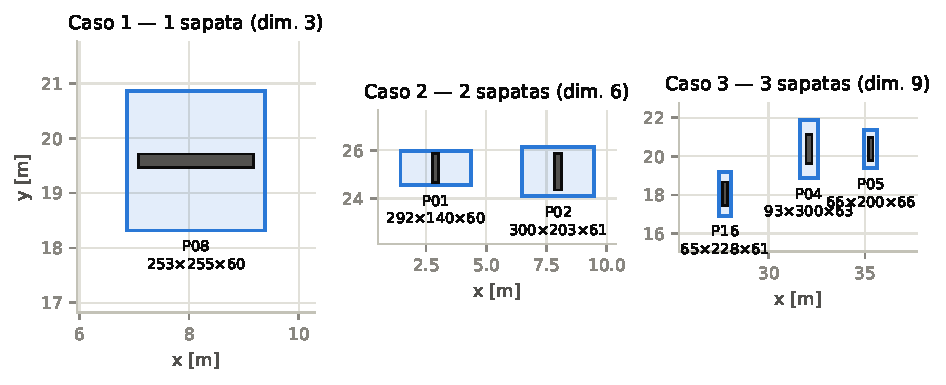
\includegraphics[width=\textwidth]{fig_planta_casos.pdf}
    \caption{Arranjo em planta da melhor solução estritamente factível do EGO por caso (retângulos claros: sapatas otimizadas; retângulos escuros: pilares; dimensões $h_x \times h_y \times h_z$ em centímetros). Reproduzido deterministicamente a partir da semente da repetição vencedora.}
    \label{fig:planta}
\end{figure*}

\subsection{Efeito do fator de penalidade no modelo substituto}
\label{sec:res_penalidade}

Para isolar o efeito do fator $\alpha$ da Equação~\eqref{eq:penalizacao} sobre a qualidade do modelo substituto, a mesma amostra de 900 pontos LHS do caso de três sapatas foi rotulada duas vezes — com $\alpha = 10^{1}$ (padrão do projeto) e $\alpha = 10^{6}$ — e particionada em treino/teste (70\%/30\%) em três réplicas independentes de amostragem e partição. Os 21 \textit{kernels} do conjunto experimental foram ajustados sob o mesmo \textit{pipeline} de produção (\textit{StandardScaler} seguido de GPR com \texttt{normalize\_y}, \textit{jitter} $10^{-1}$ e cinco reinícios do otimizador de verossimilhança).

O resultado central está na Tabela~\ref{tab:gpr_kernels} e na Figura~\ref{fig:gpr_obs_pred}, e é mais sutil do que a formulação preliminar desta pesquisa sugeria: o coeficiente $R^2$ \textit{global} é praticamente insensível à penalidade (medianas de $0{,}925$ sob $\alpha = 10^{1}$ e $0{,}919$ sob $\alpha = 10^{6}$), pois trata-se de métrica invariante à escala — sob $\alpha = 10^{6}$, a variância do alvo passa a ser dominada pelo próprio termo de penalização, e o modelo substituto reproduz essa variância artificial. O erro absoluto, contudo, muda de natureza: o RMSE global salta de $\approx \SI{2,0}{\meter\cubed}$ para $\approx 1{,}9 \times 10^{5}\,\si{\meter\cubed}$. A métrica decisiva para a otimização é o erro restrito à \textit{região factível} — onde os rótulos das duas penalidades coincidem exatamente e onde a função de aquisição precisa discriminar candidatos. Nessa região, o RMSE do \textit{kernel} de produção é de \SI{1,28}{\meter\cubed} sob $\alpha = 10^{1}$ contra $\approx 1{,}2 \times 10^{5}\,\si{\meter\cubed}$ sob $\alpha = 10^{6}$ — cinco ordens de grandeza acima da escala do volume ($\Theta \sim 10^{0}$--$10^{1}\,\si{\meter\cubed}$). Em síntese: penalidades elevadas não degradam o ajuste \textit{aparente} do GPR, mas reduzem sua utilidade exatamente onde a busca decide, o que fundamenta a adoção de penalidade moderada nesta arquitetura.

\begin{figure*}[!t]
    \centering
    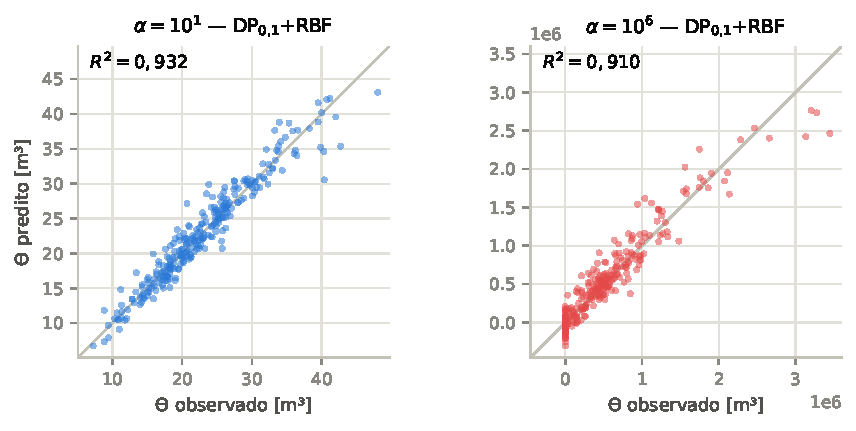
\includegraphics[width=\textwidth]{fig_gpr_obs_pred.pdf}
    \caption{Valores observados e preditos de $\Theta$ no conjunto de teste (réplica de semente 101, \textit{kernel} de melhor $R^2$ médio): sob $\alpha = 10^{6}$ (direita), a escala do alvo é dominada pela penalização ($10^{6}\,\si{\meter\cubed}$) e a região factível colapsa junto à origem, embora o $R^2$ global permaneça alto.}
    \label{fig:gpr_obs_pred}
\end{figure*}

% Gerada por scripts/make_paper_artifacts.py — nao editar manualmente.
\begin{table*}[!t]
    \centering
    \caption{Qualidade preditiva do GPR por \textit{kernel} (média em 3 réplicas independentes de amostragem/partição; caso de 3 sapatas; 900 amostras LHS; partição 70/30): as oito melhores configurações sob $\alpha = 10^{1}$ e o \textit{kernel} de produção. RMSE$_{\mathrm{feas}}$ é o erro restrito aos pontos de teste factíveis — a região onde a função de aquisição decide.}
    \label{tab:gpr_kernels}
    \small
    \begin{tabular}{llccccc}
        \toprule
        & & \multicolumn{3}{c}{$\alpha = 10^{1}$} & \multicolumn{2}{c}{$\alpha = 10^{6}$} \\
        \cmidrule(lr){3-5} \cmidrule(lr){6-7}
        Id & \textit{Kernel} & $R^2$ & RMSE & RMSE$_{\mathrm{feas}}$ & $R^2$ & RMSE$_{\mathrm{feas}}$ \\
        \midrule
        k12 & DP$_{0{,}1}$+RBF & 0,934 $\pm$ 0,010 & 1,89 & 1,26 & 0,925 & \num{1.18e+05} \\
        k10 & DP+RBF & 0,934 $\pm$ 0,010 & 1,89 & 1,26 & 0,925 & \num{1.18e+05} \\
        k07 & RQ $\alpha{=}1$ & 0,933 $\pm$ 0,011 & 1,90 & 1,25 & 0,924 & \num{1.16e+05} \\
        k09 & RQ $\alpha{=}10$ & 0,933 $\pm$ 0,011 & 1,90 & 1,25 & 0,924 & \num{1.16e+05} \\
        k08 & RQ $\alpha{=}0{,}1$ & 0,933 $\pm$ 0,011 & 1,90 & 1,25 & 0,924 & \num{1.16e+05} \\
        k19 & RQ+White & 0,933 $\pm$ 0,011 & 1,90 & 1,25 & 0,924 & \num{1.16e+05} \\
        k01 & RBF+RBF & 0,931 $\pm$ 0,012 & 1,93 & 1,24 & 0,923 & \num{1.15e+05} \\
        k06 & Matérn $1{,}5{+}2{,}5$ & 0,931 $\pm$ 0,011 & 1,94 & 1,28 & 0,921 & \num{1.2e+05} \\
        k20$^\dagger$ & Matérn $\nu{=}2{,}5$ (produção) & 0,931 $\pm$ 0,011 & 1,94 & 1,28 & 0,921 & \num{1.2e+05} \\
        \bottomrule
    \end{tabular}
    \caption*{\footnotesize $^\dagger$\,\textit{kernel} adotado em produção no \fundaai{} (\texttt{constroi\_kernel()[-1]}). RMSE em \si{\meter\cubed}.}
\end{table*}


\subsection{Efeito da escolha do \textit{kernel}}
\label{sec:res_kernels}

O conjunto experimental compreende 21 configurações de \textit{kernel} (identificadas \texttt{k00} a \texttt{k20}), das quais a última — Matérn com $\nu = 2{,}5$ e limites ampliados de comprimento de escala — é a adotada em produção na ferramenta \fundaai{}. A Figura~\ref{fig:gpr_kernels} apresenta o $R^2$ médio (e amplitude em três réplicas) por configuração e penalidade. O padrão observado nuança a expectativa de que a escolha do \textit{kernel} seria determinante: 19 das 21 configurações concentram-se em uma banda estreita ($R^2 \approx 0{,}93$) dentro da variabilidade entre réplicas ($\pm 0{,}011$); apenas o \textit{kernel} puramente periódico (\texttt{k14}) e o puramente linear (\texttt{k13}) falham, por hipótese estrutural incompatível com a resposta. A configuração de produção situa-se na banda superior ($R^2 = 0{,}931 \pm 0{,}011$), a menos de $0{,}004$ do melhor valor médio observado ($0{,}934$, \texttt{k10}/\texttt{k12}). Com apenas três réplicas por configuração, o resultado deve ser lido como rastreio exploratório: para esta formulação, a escala da penalidade (Seção~\ref{sec:res_penalidade}) e a base amostral parecem mais determinantes do que a escolha fina da função de covariância dentro das famílias suaves usuais.

\begin{figure*}[!t]
    \centering
    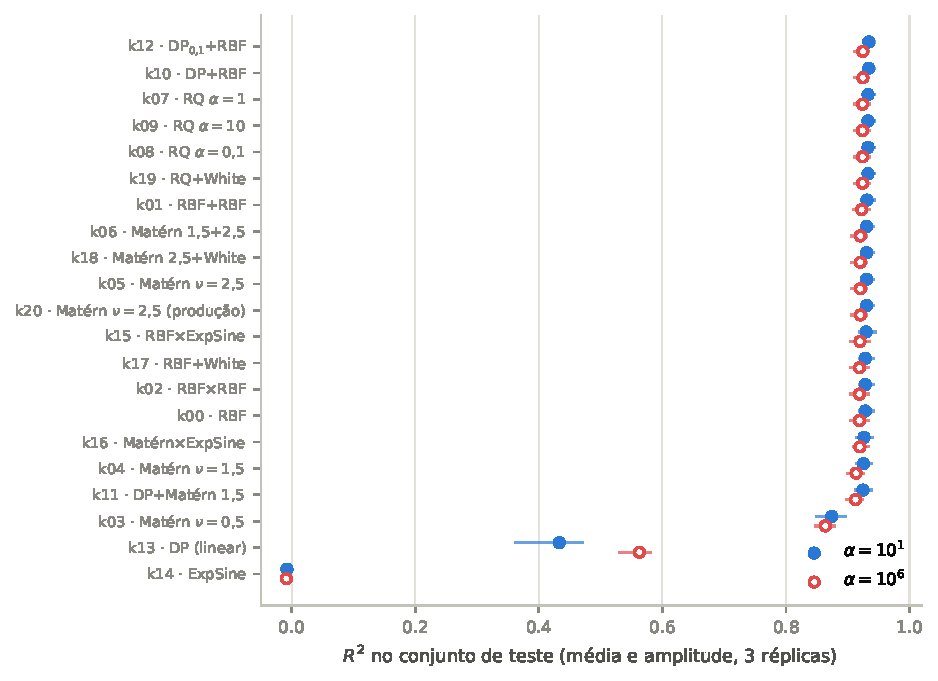
\includegraphics[width=0.78\textwidth]{fig_gpr_kernels_r2.pdf}
    \caption{$R^2$ no conjunto de teste por configuração de \textit{kernel} e fator de penalidade (média e amplitude em 3 réplicas independentes; caso de 3 sapatas). A maioria das configurações suaves fica em faixa estreita; falham apenas as hipóteses estruturais incompatíveis (periódica pura e linear pura).}
    \label{fig:gpr_kernels}
\end{figure*}

\subsection{Comparação sob orçamento igual de avaliações (cenário S1)}
\label{sec:res_s1}

A Figura~\ref{fig:convergencia} apresenta as curvas de convergência medianas (com banda interquartílica) do melhor valor de $\Theta$ em função do número de avaliações reais, e a Figura~\ref{fig:dist_best} a distribuição do melhor valor final nas 30 repetições. A Tabela~\ref{tab:s1} consolida as estatísticas e a Tabela~\ref{tab:pvalues_s1} os p-valores ajustados por Holm a partir do teste pareado de Wilcoxon bilateral sobre o melhor valor por repetição.

\begin{figure*}[!t]
    \centering
    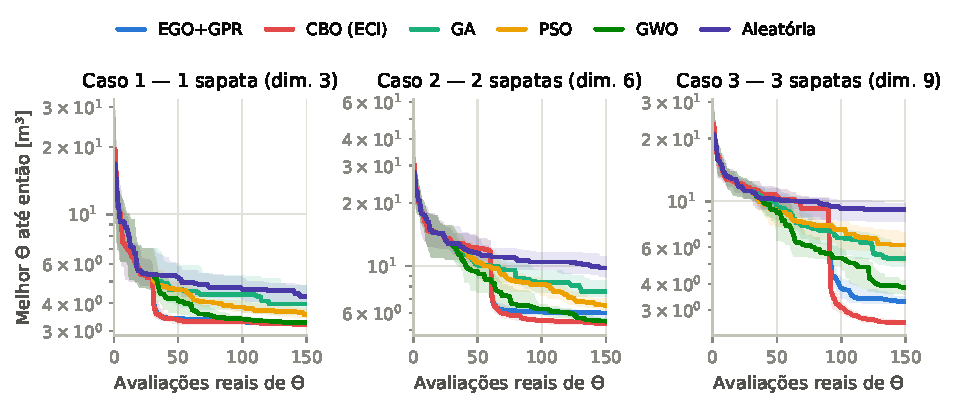
\includegraphics[width=\textwidth]{fig_convergencia_s1.pdf}
    \caption{Convergência mediana (linha) e banda interquartílica (faixa) do melhor $\Theta$ em função das avaliações reais no cenário S1. O EGO acompanha a amostragem inicial (LHS de $10d$ pontos) e reduz rapidamente $\Theta$ quando a função de aquisição EI passa a selecionar os candidatos.}
    \label{fig:convergencia}
\end{figure*}

\begin{figure*}[!t]
    \centering
    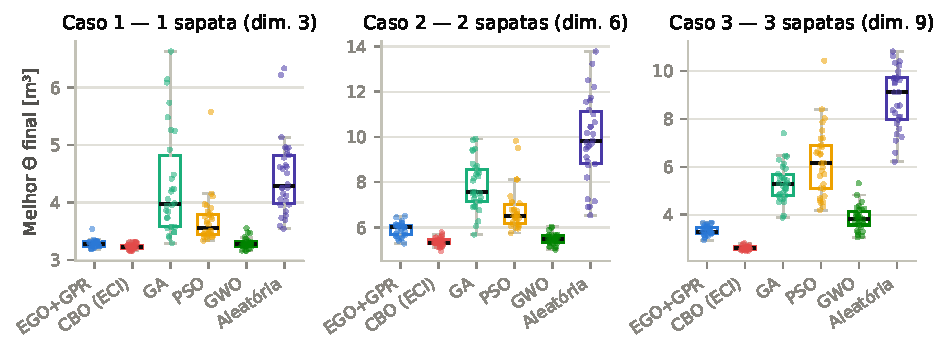
\includegraphics[width=\textwidth]{fig_dist_best_s1.pdf}
    \caption{Distribuição do melhor $\Theta$ final por algoritmo no cenário S1 (30 repetições; caixas com mediana; pontos individuais sobrepostos).}
    \label{fig:dist_best}
\end{figure*}

% Gerada por scripts/make_paper_artifacts.py — nao editar manualmente.
\begin{table*}[!t]
    \centering
    \caption{Cenário S1 (orçamento igual de 150 avaliações reais): estatísticas do melhor $\Theta$ [\si{\meter\cubed}] em 30 repetições, factibilidade da solução final (tolerância $g_k \le 10^{-9}$), violação máxima média, melhor volume factível $V^{\mathrm{feas}}_{\min}$ [\si{\meter\cubed}] e tempo de parede.}
    \label{tab:s1}
    \small
    \begin{tabular}{llccccccc}
        \toprule
        Caso & Algoritmo & Melhor & Média $\pm$ DP & Mediana & Fact. & $\overline{\max g_k}$ & $V^{\mathrm{feas}}_{\min}$ & Tempo [s] \\
        \midrule
        Caso 1 & EGO+GPR & 3,184 & 3,283 $\pm$ 0,067 & 3,285 & 83\% & 0,000 & 3,184 & 72,28 \\
        Caso 1 & CBO (ECI) & 3,159 & 3,233 $\pm$ 0,047 & 3,228 & 63\% & 0,004 & 3,159 & 115,92 \\
        Caso 1 & GA & 3,289 & 4,317 $\pm$ 0,934 & 3,973 & 57\% & 0,011 & 3,289 & 0,02 \\
        Caso 1 & PSO & 3,336 & 3,691 $\pm$ 0,424 & 3,562 & 63\% & 0,015 & 3,363 & 0,02 \\
        Caso 1 & GWO & 3,156 & 3,287 $\pm$ 0,092 & 3,278 & 63\% & 0,006 & 3,156 & 0,02 \\
        Caso 1 & Aleatória & 3,542 & 4,450 $\pm$ 0,671 & 4,287 & 47\% & 0,040 & 3,542 & 0,02 \\
        \midrule
        Caso 2 & EGO+GPR & 5,290 & 5,909 $\pm$ 0,303 & 6,004 & 83\% & 0,003 & 5,290 & 57,07 \\
        Caso 2 & CBO (ECI) & 4,959 & 5,357 $\pm$ 0,176 & 5,324 & 37\% & 0,015 & 5,107 & 89,40 \\
        Caso 2 & GA & 5,681 & 7,865 $\pm$ 1,108 & 7,578 & 53\% & 0,025 & 6,272 & 0,02 \\
        Caso 2 & PSO & 5,756 & 6,804 $\pm$ 0,961 & 6,517 & 60\% & 0,039 & 5,952 & 0,02 \\
        Caso 2 & GWO & 5,009 & 5,478 $\pm$ 0,246 & 5,482 & 50\% & 0,014 & 5,090 & 0,02 \\
        Caso 2 & Aleatória & 6,537 & 9,906 $\pm$ 1,881 & 9,809 & 30\% & 0,150 & 6,537 & 0,02 \\
        \midrule
        Caso 3 & EGO+GPR & 2,941 & 3,335 $\pm$ 0,195 & 3,289 & 83\% & 0,003 & 2,941 & 39,51 \\
        Caso 3 & CBO (ECI) & 2,490 & 2,612 $\pm$ 0,081 & 2,607 & 83\% & 0,000 & 2,490 & 61,30 \\
        Caso 3 & GA & 3,874 & 5,327 $\pm$ 0,759 & 5,286 & 53\% & 0,031 & 3,874 & 0,02 \\
        Caso 3 & PSO & 4,181 & 6,200 $\pm$ 1,420 & 6,157 & 43\% & 0,068 & 4,181 & 0,02 \\
        Caso 3 & GWO & 3,063 & 3,862 $\pm$ 0,509 & 3,837 & 60\% & 0,011 & 3,063 & 0,02 \\
        Caso 3 & Aleatória & 6,211 & 8,853 $\pm$ 1,254 & 9,108 & 37\% & 0,068 & 6,211 & 0,02 \\
        \bottomrule
    \end{tabular}
\end{table*}

% Gerada por scripts/make_paper_artifacts.py — nao editar manualmente.
\begin{table*}[!t]
    \centering
    \caption{Matriz triangular de p-valores ajustados por Holm a partir do teste pareado de Wilcoxon bilateral sobre o melhor $\Theta$ por repetição no cenário S1; valores em negrito indicam $p < 0{,}05$.}
    \label{tab:pvalues_s1}
    \small
    \begin{tabular}{lccccc}
        \toprule
         & CBO (ECI) & GA & PSO & GWO & Aleatória \\
        \midrule
        \multicolumn{6}{l}{\textit{Caso 1 — 1 sapata (dim. 3)}} \\
        \midrule
        EGO+GPR & \textbf{0,014} & \textbf{$<$0,001} & \textbf{$<$0,001} & 1,000 & \textbf{$<$0,001} \\
        CBO (ECI) &  & \textbf{$<$0,001} & \textbf{$<$0,001} & \textbf{0,014} & \textbf{$<$0,001} \\
        GA &  &  & \textbf{0,004} & \textbf{$<$0,001} & 0,316 \\
        PSO &  &  &  & \textbf{$<$0,001} & \textbf{$<$0,001} \\
        GWO &  &  &  &  & \textbf{$<$0,001} \\
        \addlinespace[6pt]
        \multicolumn{6}{l}{\textit{Caso 2 — 2 sapatas (dim. 6)}} \\
        \midrule
        EGO+GPR & \textbf{$<$0,001} & \textbf{$<$0,001} & \textbf{$<$0,001} & \textbf{$<$0,001} & \textbf{$<$0,001} \\
        CBO (ECI) &  & \textbf{$<$0,001} & \textbf{$<$0,001} & \textbf{0,029} & \textbf{$<$0,001} \\
        GA &  &  & \textbf{0,001} & \textbf{$<$0,001} & \textbf{$<$0,001} \\
        PSO &  &  &  & \textbf{$<$0,001} & \textbf{$<$0,001} \\
        GWO &  &  &  &  & \textbf{$<$0,001} \\
        \addlinespace[6pt]
        \multicolumn{6}{l}{\textit{Caso 3 — 3 sapatas (dim. 9)}} \\
        \midrule
        EGO+GPR & \textbf{$<$0,001} & \textbf{$<$0,001} & \textbf{$<$0,001} & \textbf{$<$0,001} & \textbf{$<$0,001} \\
        CBO (ECI) &  & \textbf{$<$0,001} & \textbf{$<$0,001} & \textbf{$<$0,001} & \textbf{$<$0,001} \\
        GA &  &  & \textbf{0,013} & \textbf{$<$0,001} & \textbf{$<$0,001} \\
        PSO &  &  &  & \textbf{$<$0,001} & \textbf{$<$0,001} \\
        GWO &  &  &  &  & \textbf{$<$0,001} \\
        \bottomrule
    \end{tabular}
\end{table*}


Quatro padrões emergem. Primeiro, \textbf{o CBO apresenta a melhor média e a melhor mediana de $\Theta$ nos três casos avaliados}, com vantagem significativa sobre EGO, AG, PSO, GWO e busca aleatória nas matrizes pareadas da Tabela~\ref{tab:pvalues_s1}, exceto pelo confronto EGO--GWO no caso 1, em que há empate estatístico. Segundo, \textbf{a redução mediana da melhor arquitetura assistida em relação à busca aleatória aumenta na sequência dos casos testados}: $24{,}7\,\%$ no caso 1, $45{,}7\,\%$ no caso 2 e $71{,}4\,\%$ no caso 3; para o EGO penalizado isoladamente, as reduções são $23{,}4\,\%$, $38{,}8\,\%$ e $63{,}9\,\%$. Como há uma instância por dimensionalidade e a restrição de sobreposição está inativa, esse padrão é interpretado como evidência nas instâncias avaliadas, não como isolamento causal do efeito da dimensão. Terceiro, \textbf{as arquiteturas assistidas são também as mais estáveis}, especialmente o CBO, cujos desvios-padrão são $0{,}047$, $0{,}176$ e $0{,}081\,\si{\meter\cubed}$ nos três casos.

O quarto padrão é o confronto que isola o tratamento das restrições: \textbf{o CBO melhora $\Theta$ em relação ao EGO nos três casos, mas troca parte dessa melhoria por perda de factibilidade nos casos 1 e 2}. A média de $\Theta$ do CBO fica $1{,}5\,\%$, $9{,}3\,\%$ e $21{,}7\,\%$ abaixo da média do EGO nos casos 1--3, respectivamente. Em melhor volume estritamente factível, o CBO também melhora o EGO em $0{,}8\,\%$, $3{,}5\,\%$ e $15{,}3\,\%$. Contudo, as taxas de factibilidade estrita são $63\,\%$, $37\,\%$ e $83\,\%$ no CBO, contra $83\,\%$ em todos os casos para o EGO. Esse comportamento é coerente com a mecânica do método: quando a restrição ativa é suave e o ótimo encosta na fronteira de tensão, os GPs de restrição podem superestimar localmente a probabilidade de factibilidade. Nas instâncias avaliadas, o CBO explora essa fronteira de forma mais agressiva, enquanto o EGO penalizado preserva maior regularidade de factibilidade; a validação desse padrão em problemas realmente acoplados fica reservada à frente de posicionamento conjunto. O custo computacional do CBO é o esperado de múltiplos modelos substitutos por iteração: cerca de $1{,}5$ a $1{,}6$ vez o tempo de parede do EGO por repetição.

\subsection{Orçamento estendido e tempo de parede (cenário S2)}
\label{sec:res_s2}

O cenário S2 responde à pergunta complementar: quando a avaliação de $\Theta$ tem baixo custo computacional, o que as buscas diretas entregam com orçamento folgado? A Tabela~\ref{tab:s2} e a Figura~\ref{fig:s1s2} mostram que, com $3\,000$ avaliações ($20\times$ o orçamento de S1), PSO e GWO superam consistentemente as referências assistidas por modelo substituto de 150 avaliações — no caso 3, o GWO atinge $2{,}200 \pm 0{,}022\,\si{\meter\cubed}$ contra $3{,}335 \pm 0{,}195\,\si{\meter\cubed}$ do EGO--150 e $2{,}612 \pm 0{,}081\,\si{\meter\cubed}$ do CBO--150 — consumindo, contudo, apenas $0{,}3$--$0{,}4$ segundos de parede por repetição, contra dezenas de segundos dos métodos assistidos. O custo de parede do EGO/CBO é dominado pelo próprio método (ajustes sucessivos de GPR e maximização interna da aquisição), não pelas avaliações de $\Theta$, que respondem por menos de $0{,}1\,\%$ do tempo total. Esses dois regimes delimitam com precisão o domínio de adequação da arquitetura: \textbf{as arquiteturas assistidas são competitivas quando o orçamento de avaliações reais é o recurso escasso; as buscas diretas são preferíveis quando o recurso escasso é o tempo de parede e a avaliação tem baixo custo}. O resultado do caso 3 indica ainda que 150 avaliações são insuficientes para esgotar o problema de nove variáveis (o teto prático observado situa-se em torno de $2{,}17$--$2{,}20\,\si{\meter\cubed}$), delimitando o orçamento adotado como escolha de protocolo, e não como capacidade máxima do método.

\begin{figure*}[!t]
    \centering
    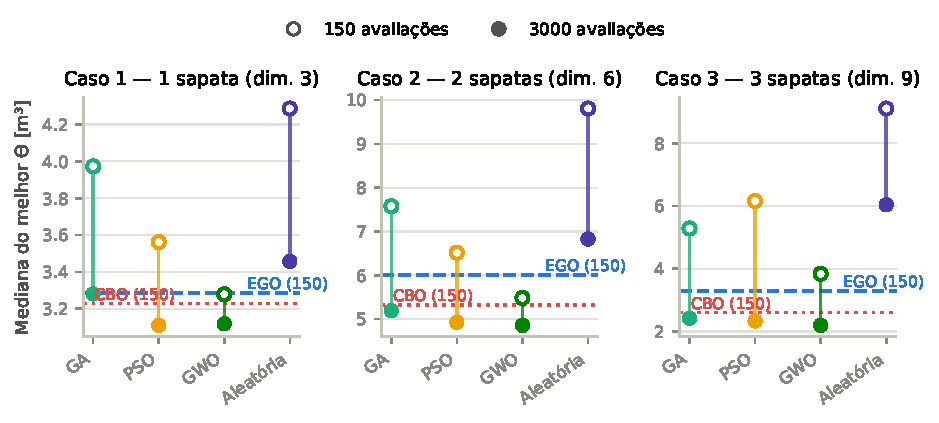
\includegraphics[width=\textwidth]{fig_s1_vs_s2.pdf}
    \caption{Mediana do melhor $\Theta$ por algoritmo sob 150 avaliações (círculos vazados) e $3\,000$ avaliações (círculos cheios), com a referência EGO--150 (linha tracejada). Com avaliação de baixo custo e orçamento estendido, as buscas diretas ultrapassam a referência em menor tempo de parede.}
    \label{fig:s1s2}
\end{figure*}

% Gerada por scripts/make_paper_artifacts.py — nao editar manualmente.
\begin{table*}[!t]
    \centering
    \caption{Cenário S2 (orçamento estendido de 3\,000 avaliações reais para as buscas diretas): estatísticas em 30 repetições, mesmas \textit{seeds} do S1.}
    \label{tab:s2}
    \small
    \begin{tabular}{llccccccc}
        \toprule
        Caso & Algoritmo & Melhor & Média $\pm$ DP & Mediana & Fact. & $\overline{\max g_k}$ & $V^{\mathrm{feas}}_{\min}$ & Tempo [s] \\
        \midrule
        Caso 1 & GA & 3,134 & 3,352 $\pm$ 0,189 & 3,280 & 60\% & 0,002 & 3,145 & 0,40 \\
        Caso 1 & PSO & 3,109 & 3,115 $\pm$ 0,024 & 3,109 & 60\% & 0,000 & 3,109 & 0,36 \\
        Caso 1 & GWO & 3,110 & 3,118 $\pm$ 0,004 & 3,118 & 57\% & 0,000 & 3,110 & 0,37 \\
        Caso 1 & Aleatória & 3,129 & 3,431 $\pm$ 0,112 & 3,457 & 60\% & 0,008 & 3,129 & 0,31 \\
        \midrule
        Caso 2 & GA & 4,906 & 5,271 $\pm$ 0,230 & 5,191 & 53\% & 0,002 & 5,029 & 0,43 \\
        Caso 2 & PSO & 4,769 & 4,945 $\pm$ 0,105 & 4,927 & 47\% & 0,000 & 4,834 & 0,39 \\
        Caso 2 & GWO & 4,776 & 4,867 $\pm$ 0,054 & 4,855 & 53\% & 0,001 & 4,787 & 0,40 \\
        Caso 2 & Aleatória & 5,642 & 6,841 $\pm$ 0,680 & 6,828 & 47\% & 0,028 & 5,774 & 0,34 \\
        \midrule
        Caso 3 & GA & 2,288 & 2,429 $\pm$ 0,095 & 2,421 & 63\% & 0,001 & 2,331 & 0,44 \\
        Caso 3 & PSO & 2,166 & 2,409 $\pm$ 0,242 & 2,336 & 60\% & 0,001 & 2,203 & 0,39 \\
        Caso 3 & GWO & 2,167 & 2,200 $\pm$ 0,022 & 2,195 & 70\% & 0,000 & 2,167 & 0,41 \\
        Caso 3 & Aleatória & 4,651 & 5,991 $\pm$ 0,667 & 6,039 & 63\% & 0,025 & 4,651 & 0,35 \\
        \bottomrule
    \end{tabular}
\end{table*}


\subsection{Diagnóstico de quase separabilidade por decomposição}
\label{sec:res_decomposicao}

A observação geométrica da Seção~\ref{sec:res_casos} tem consequência direta: como a restrição de sobreposição é inativa nos três casos congelados, o problema atual se aproxima da soma de subproblemas independentes de três variáveis, um por sapata. Para quantificar esse efeito, cada sapata foi otimizada separadamente por Differential Evolution com critério auxiliar de factibilidade, as soluções locais foram concatenadas e o vetor completo foi reavaliado pelo mesmo avaliador global usado no protocolo. A Tabela~\ref{tab:decomposicao} mostra que essa decomposição produz soluções estritamente factíveis e melhora o melhor volume factível já observado no protocolo global em $<0{,}01\,\%$, $0{,}77\,\%$ e $2{,}08\,\%$ nos casos 1--3, respectivamente.

% Gerada por scripts/make_paper_artifacts.py — nao editar manualmente.
\begin{table*}[!t]
    \centering
    \caption{Diagnóstico de quase separabilidade: baseline de Differential Evolution aplicado separadamente a cada sapata, seguido de reavaliação global estrita pelo mesmo avaliador de $\Theta$. A redução é calculada contra o melhor volume estritamente factível já obtido no protocolo global (S1/S2); portanto, a tabela mede proximidade estrutural ao ótimo das instâncias simplificadas, não desempenho pareado sob orçamento igual.}
    \label{tab:decomposicao}
    \small
    \begin{tabular}{lclccccc}
        \toprule
        Caso & Dim. & $V_{\mathrm{dec}}$ & Melhor protocolo & $V_{\mathrm{prot}}$ & Redução & $\max g_k$ & Avaliações \\
        \midrule
        Caso 1 & 3 & 3,109 & PSO (S2) & 3,109 & $<$0,01\% & \num{0.0e+00} & 11124 \\
        Caso 2 & 6 & 4,751 & GWO (S2) & 4,787 & 0,77\% & \num{0.0e+00} & 24588 \\
        Caso 3 & 9 & 2,122 & GWO (S2) & 2,167 & 2,08\% & \num{0.0e+00} & 35964 \\
        \bottomrule
    \end{tabular}
    \caption*{\footnotesize Volumes em \si{\meter\cubed}. O baseline usa penalização de factibilidade apenas para guiar a busca local; os valores reportados são volumes reavaliados e factíveis com tolerância $g_k \le 10^{-9}$.}
\end{table*}


O resultado tem duas implicações metodológicas. Primeiro, ele confirma que os casos atuais são adequados para testar integração de código, penalização, CBO e eficiência amostral, mas ainda não exercitam fortemente o acoplamento geométrico entre fundações. Segundo, ele impede uma leitura excessiva do aumento de ganho com a dimensionalidade: parte do desempenho observado decorre de resolver várias sapatas quase independentes, não necessariamente de uma vantagem intrínseca dos modelos substitutos em problemas acoplados de maior dimensão. Por isso, o artigo trata a decomposição como auditoria estrutural do problema atual e remete a validação de problemas não separáveis à frente de posicionamento conjunto.

\subsection{Factibilidade das soluções finais e comportamento da penalização}
\label{sec:res_factibilidade}

A aferição estrita de factibilidade ($g_k \le 10^{-9}$) expõe um comportamento previsto pela teoria da penalização exterior com fator finito: em todos os algoritmos guiados por $\Theta$, parte das soluções finais carrega violações residuais — tipicamente da ordem de $10^{-4}$ a $10^{-1}$ na razão normalizada $g_k$ —, pois, com $\alpha = 10$ e penalização linear ($p = 1$), uma violação marginal que economize volume superior a $10\,g_k$ é aceita pelo otimizador. A Figura~\ref{fig:violacoes} apresenta a violação máxima por solução final: entre os métodos guiados pela penalização, o EGO manteve a maior regularidade de factibilidade no cenário S1 ($83\,\%$ nos três casos), com melhores volumes estritamente factíveis de \SI{3,184}{\meter\cubed}, \SI{5,290}{\meter\cubed} e \SI{2,941}{\meter\cubed}. O CBO, único método que otimiza a factibilidade explicitamente, reduziu esses volumes para \SI{3,159}{\meter\cubed}, \SI{5,107}{\meter\cubed} e \SI{2,490}{\meter\cubed}, mas com factibilidade de $63\,\%$, $37\,\%$ e $83\,\%$, respectivamente. Quanto às restrições governantes, a análise das soluções finais confirma e refina o padrão qualitativo das etapas anteriores: a tensão admissível do solo é a restrição ativa nos três casos ($S/R \to 1$); as duas verificações de punção permanecem folgadas na faixa explorada; e, no caso 1, a compatibilidade geométrica é estruturalmente ativa na direção $x$, pois o pilar de $a_p = \SI{2,10}{\meter}$ impõe $h_x \ge \SI{2,30}{\meter}$. Esses resultados quantificam o compromisso embutido na estratégia de penalização adotada e motivam, como refinamento futuro, esquemas de tratamento explícito de restrições e seleção final por dominância de factibilidade (Seção~\ref{sec:conclusoes}).

\begin{figure*}[!t]
    \centering
    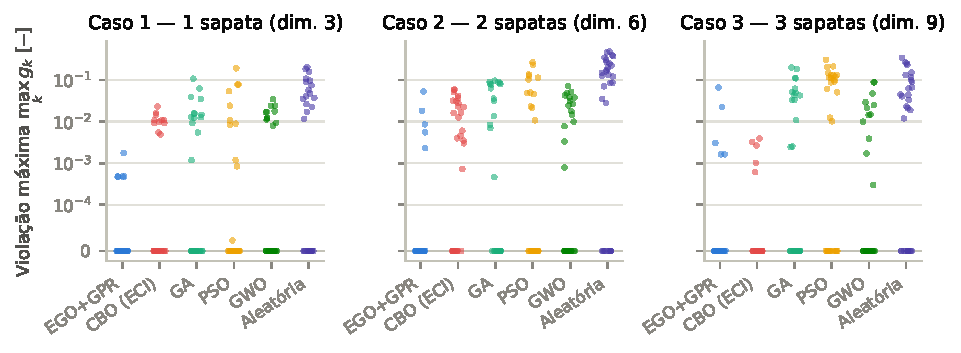
\includegraphics[width=\textwidth]{fig_violacoes_s1.pdf}
    \caption{Violação máxima de restrição da melhor solução de cada repetição (cenário S1; escala simétrico-logarítmica; valores no eixo do zero correspondem a soluções estritamente factíveis). A penalização exterior linear com $\alpha = 10$ admite violações residuais em todos os métodos.}
    \label{fig:violacoes}
\end{figure*}

% =============================================================================
% Seção 7 — Discussão
% =============================================================================
\section{Discussão}
\label{sec:discussao}

Os resultados da Seção~\ref{sec:resultados} podem ser discutidos sob quatro eixos complementares: a adequação do EGO à formulação atual, o desempenho preditivo do modelo substituto, o comportamento da penalização exterior e as limitações estruturais da formulação implementada.

\paragraph{Adequação do EGO à formulação atual: dois regimes bem delimitados.}
O EGO é classicamente justificado em problemas de otimização tipo caixa-preta com avaliações de alto custo computacional \citepabnt{jones1998efficient}. A função pseudo-objetivo $\Theta$ desta formulação, entretanto, tem baixo custo na implementação vetorizada atual ($\approx \SI{0,1}{\milli\second}$ por avaliação), o que torna a justificativa clássica insuficiente e exige avaliação empírica explícita. O protocolo de dois cenários responde à questão com precisão. Sob \textit{orçamento igual de avaliações reais} (S1), as arquiteturas assistidas por modelo substituto reduzem $\Theta$ frente às buscas não assistidas, e o CBO apresenta as melhores médias nos três casos. Sob \textit{tempo de parede} com avaliação de baixo custo (S2), buscas diretas com orçamento estendido entregam soluções melhores em duas ordens de grandeza menos tempo, pois o custo do EGO/CBO é dominado pelos ajustes sucessivos do GPR e pela maximização interna da aquisição. A auditoria por decomposição (Tabela~\ref{tab:decomposicao}) acrescenta uma terceira leitura: nas instâncias simplificadas atuais, uma linha de base por sapata praticamente atinge ou supera o melhor volume factível global, confirmando que o problema ainda não explora o acoplamento que justificará plenamente a arquitetura assistida. A adoção do EGO nesta etapa deve, portanto, ser lida como investimento metodológico deliberado: a arquitetura é candidata natural para extensões em que cada avaliação se tornará genuinamente custosa — posicionamento conjunto com empacotamento, interação entre bulbos de tensão, recalques e eventuais acoplamentos numéricos —, mas não é uma necessidade computacional da formulação algébrica atual. Essa leitura é coerente com \citeonline{mathern2021multiobjective}, que exploram em projeto estrutural uma assimetria entre objetivos de baixo custo e restrições normativas mais custosas, cenário ainda não plenamente ativado no recorte atual do FundaIA.

\paragraph{Sensibilidade ao fator de penalidade: o que o $R^2$ esconde.}
O estudo controlado de penalidade refina o diagnóstico das etapas preliminares desta pesquisa. A constatação original — de que penalidades elevadas degradam o ajuste do GPR — mostrou-se imprecisa quando aferida por $R^2$ global: sob $\alpha = 10^{6}$, a variância do alvo é dominada pelo próprio termo de penalização e o $R^2$ permanece alto ($\approx 0{,}92$), mascarando o problema. A métrica reveladora é o erro absoluto na \textit{região factível}, onde a função de aquisição efetivamente discrimina candidatos: ali, o RMSE sob $\alpha = 10^{6}$ é cerca de cinco ordens de grandeza superior à escala do volume, contra $\approx 1{,}3\,\si{\meter\cubed}$ sob $\alpha = 10^{1}$. A consequência prática é direta: com penalidade agressiva, a EI passa a ser governada pelo gradiente artificial da penalização, e não pela paisagem do volume. Esse resultado fundamenta quantitativamente a adoção de penalidade moderada na arquitetura penalizada — e motivou a implementação, nesta mesma pesquisa, da alternativa que remove a penalização de todos os alvos de regressão: a \textit{Constrained Bayesian Optimization} da Seção~\ref{sec:met_cbo}, discutida a seguir.

\paragraph{Tratamento explícito de restrições: quando compensa.}
O confronto pareado CBO~$\times$~EGO — idênticos em tudo, exceto no tratamento das restrições — produziu um resultado assimétrico: o CBO melhora $\Theta$ nos três casos, mas perde factibilidade estrita nos casos 1 e 2. A explicação é coerente com a mecânica dos dois métodos: com o ótimo encostado na fronteira de tensão e poucas observações, o GP da restrição suaviza o cruzamento do zero e a probabilidade de factibilidade da Equação~\eqref{eq:pof} pode superestimar a margem — um erro \textit{de modelo}; já a penalização direta com fator finito desloca o ótimo penalizado em relação ao ótimo restrito — um erro \textit{de formulação}. Como há apenas uma instância por dimensionalidade e a restrição de sobreposição está inativa, o resultado não demonstra isoladamente que o ganho decorre da dimensão. Ele indica, de forma mais cautelosa, que o tratamento explícito de restrições merece prioridade na próxima fase, desde que acompanhado por regras de seleção final estritamente factíveis; no regime de posicionamento conjunto ($5N$ variáveis), a restrição de sobreposição se tornará ativa e produzirá acoplamento real entre fundações. Nesse regime, variantes escaláveis com regiões de confiança \citepabnt{eriksson2021scbo} são o caminho declarado quando $N$ crescer.

\paragraph{Escolha do \textit{kernel}: menos decisiva do que se supunha.}
O rastreio controlado de 21 configurações mostrou que 19 delas se concentram em faixa estreita de capacidade preditiva ($R^2 \approx 0{,}93 \pm 0{,}011$), falhando apenas as hipóteses estruturais incompatíveis com a resposta (periódica pura e linear pura). Esse achado é coerente com a interpretação de \citeonline{schulz2018tutorial} — a função de covariância codifica hipóteses de regularidade — mas deve ser interpretado como triagem exploratória, pois apenas três réplicas foram usadas por configuração. Para esta formulação, a escolha fina do \textit{kernel} dentro das famílias suaves usuais parece importar menos do que a escala da penalidade e o tamanho da base amostral. A configuração de produção (Matérn $\nu = 2{,}5$) situa-se na banda superior, e não há evidência prática que justifique substituí-la sem um estudo maior.

\paragraph{Ganho sobre buscas não assistidas e leitura de engenharia.}
Sob o mesmo orçamento de 150 avaliações reais, a redução mediana da melhor arquitetura assistida em relação à busca aleatória uniforme foi de $24{,}7\,\%$, $45{,}7\,\%$ e $71{,}4\,\%$ nos casos 1, 2 e 3, respectivamente; para o EGO penalizado isoladamente, as reduções foram $23{,}4\,\%$, $38{,}8\,\%$ e $63{,}9\,\%$. Esses números substituem, agora com sementes pareadas, orçamento equalizado e teste estatístico pareado, a comparação exploratória com Monte Carlo das etapas preliminares. Cabe a ressalva metodológica já assumida anteriormente: a busca aleatória é um piso de referência, não uma representação da prática profissional, na qual heurísticas de pré-dimensionamento aproximam o ponto de partida de regiões viáveis \citepabnttwo{wang2008economic}{waheed2022practical}. A leitura de engenharia dos arranjos finais é coerente com a formulação adotada: a tensão admissível governa os três casos ($S/R \to 1$), a punção nos contornos $C$ e $C'$ permanece folgada na faixa explorada e, no caso 1, a geometria do pilar alongado ($a_p = \SI{2,10}{\meter}$) ativa a restrição de balanço mínimo na direção $x$.

\paragraph{Penalização linear e factibilidade estrita.}
A aferição com tolerância estrita expôs o compromisso estrutural da penalização exterior com fator finito: soluções finais de todos os métodos carregam violações residuais ($g_k \sim 10^{-3}$--$10^{-1}$), pois o ótimo do problema penalizado com $\alpha = 10$ e $p = 1$ não coincide exatamente com o ótimo restrito. Essas violações não devem ser aceitas como soluções de projeto, nem interpretadas como absorvidas por coeficientes parciais de segurança. Elas importam metodologicamente por três razões: (i) quantificam o efeito previsto pela teoria clássica de penalização; (ii) mostram que a avaliação por $\Theta$ precisa ser acompanhada por métricas de factibilidade e melhor volume estritamente factível; e (iii) estabelecem a linha de base contra a qual esquemas alternativos — penalização adaptativa, regras de factibilidade de Deb, seleção final por dominância de factibilidade e \textit{Constrained Bayesian Optimization} — deverão ser julgados na continuidade da pesquisa.

\paragraph{Limitações da formulação atual.}
Cinco limitações delimitam o alcance das conclusões e motivam os trabalhos futuros da Seção~\ref{sec:conclusoes}:
\begin{enumerate}
    \item \textbf{Posições fixas e quase separabilidade.} As posições $(x_g, y_g)$ são dados de entrada; nos três casos congelados, a restrição de não sobreposição é inativa por construção. Assim, o problema conjunto de $N_{\mathrm{f}}$ sapatas é quase separável em subproblemas tridimensionais. A linha de base por decomposição já quantifica esse efeito e mostra que os melhores volumes factíveis globais estão próximos do ótimo decomposto; logo, os ganhos com o aumento de $N_{\mathrm{f}}$ não podem ser atribuídos causalmente à dimensionalidade.
    \item \textbf{Pré-dimensionamento, não projeto executivo.} A punção é verificada nos dois contornos críticos da NBR~6118 ($C$ e $C'$, este a $2d$ da face, com transferência de momentos), mas a ferramenta não dimensiona armadura de flexão, não verifica cisalhamento unidirecional, não trata ancoragem/detalhamento e não calcula custo total. Essa diferença é material: trabalhos de otimização de sapatas voltados a projeto econômico normalmente incluem armadura, custo e verificações estruturais adicionais \citepabnttwo{nigdeli2018metaheuristic}{waheed2022practical}. A taxa $\rho$ que alimenta $\tau_{Rd1}$ é a mínima normativa, adotada como hipótese de modelagem \citepabnttwo{waheed2022practical}{santos2018punching}.
    \item \textbf{Simplificações geotécnicas e de ações.} A correlação $N_{\mathrm{spt}}$--$\sigma_{\mathrm{adm}}$ permanece como hipótese empírica de pré-dimensionamento. Estudos recentes tratam capacidade de carga e recalque de fundações superficiais por modelos de dados calibrados \citepabnttwo{ahmad2021gpr}{khajehzadeh2022effective}, e \citeonline{fattahi2025settlement} destacam a sensibilidade de previsões de recalque ao SPT; tais trabalhos reforçam que a correlação simples usada aqui não deve ser lida como validação geotécnica final. A formulação de tensões já calcula o peso próprio como função explícita do volume e não aplica os coeficientes legados de $1{,}05$ e $1{,}30$ na comparação com $\sigma_{\mathrm{adm}}$, mas ainda é necessário separar formalmente combinações de serviço e de estado limite último em uma etapa de projeto completo.
    \item \textbf{Independência geotécnica.} Interações por bulbo de tensões, recalques diferenciais e variabilidade geotécnica não são modeladas \citepabnt{juang2013reliability}.
    \item \textbf{Orçamento e generalização.} As conclusões de S1 valem para o regime de 150 avaliações nas três instâncias avaliadas; o caso 3 indica que esse orçamento não esgota o problema, e a extrapolação para dimensionalidades maiores requer novo experimento.
\end{enumerate}

\paragraph{Reprodutibilidade.}
Em alinhamento com a literatura de comparação rigorosa de metaheurísticas \citepabnttwo{gomes2018probabilistic}{morales2020balance}, o protocolo final adotou 30 repetições semeadas por célula experimental, sementes pareadas entre algoritmos, orçamento de avaliações equalizado por cenário, teste não paramétrico pareado com correção para múltiplas comparações e persistência integral de configurações, históricos por avaliação, métricas e metadados de ambiente (versões de bibliotecas e revisão do repositório), com todas as figuras e tabelas regeneráveis por \textit{scripts} determinísticos. A extensão natural do desenho experimental — inclusão de CMA-ES, Differential Evolution como método pareado de orçamento controlado, linhas de base determinísticas e réplicas em problemas de maior porte — permanece como continuidade; em particular, \citeonline{nigdeli2018metaheuristic} reforçam a utilidade de comparar algoritmos não apenas por melhor valor, mas também por média, dispersão e esforço de avaliação em problemas de sapatas.

% =============================================================================
% Seção 8 — Conclusões e trabalhos futuros
% =============================================================================
\section{Conclusões e trabalhos futuros}
\label{sec:conclusoes}

Este artigo apresentou uma abordagem computacional para o pré-dimensionamento geométrico de fundações superficiais do tipo sapata isolada, formulada como otimização mono-objetivo penalizada e resolvida por uma arquitetura híbrida \textit{Efficient Global Optimization} (EGO) com modelo substituto por Regressão por Processos Gaussianos (GPR) e Algoritmo Genético (AG) como otimizador interno da função de aquisição \textit{Expected Improvement} (EI). O recorte corresponde à primeira frente metodológica do plano de trabalho — dimensões de sapatas com posições de pilares fornecidas pelo projeto estrutural e verificações parciais de tensão, geometria e punção —, agora sustentado por um protocolo experimental fechado: 30 repetições semeadas por célula, orçamento de avaliações equalizado, dois cenários de comparação, teste estatístico pareado e artefatos integralmente persistidos e regeneráveis.

As conclusões consolidadas são as seguintes:
\begin{enumerate}
    \item \textbf{Eficiência amostral demonstrada nas instâncias avaliadas.} Sob orçamento igual de 150 avaliações reais, as arquiteturas assistidas por modelo substituto ocupam o topo em $\Theta$ nos três casos. A redução mediana da melhor arquitetura assistida em relação à busca aleatória foi de $24{,}7\,\%$, $45{,}7\,\%$ e $71{,}4\,\%$ na sequência de casos testada; para o EGO isolado, foi de $23{,}4\,\%$, $38{,}8\,\%$ e $63{,}9\,\%$. Como há uma instância por dimensionalidade e a restrição de sobreposição permanece inativa, esse padrão não deve ser interpretado como isolamento causal do efeito da dimensão.
    \item \textbf{A quase separabilidade foi quantificada, não apenas declarada.} A linha de base por Differential Evolution por sapata, seguida de reavaliação global estrita, encontrou volumes factíveis de \SI{3,109}{\meter\cubed}, \SI{4,751}{\meter\cubed} e \SI{2,122}{\meter\cubed}. Esses valores empatam ou melhoram o melhor volume factível obtido no protocolo global em $<0{,}01\,\%$, $0{,}77\,\%$ e $2{,}08\,\%$, respectivamente. Portanto, os casos atuais são fortes para validar implementação, métricas, penalização e CBO, mas ainda fracos para demonstrar comportamento em problemas acoplados.
    \item \textbf{O tratamento explícito de restrições melhora $\Theta$, mas exige seleção factível.} A \textit{Constrained Bayesian Optimization} (CBO), que modela volume e restrições por modelos substitutos independentes com aquisição por probabilidade de factibilidade \citepabnt{gardner2014bayesian}, foi confrontada com o EGO penalizado sob sementes, orçamento e demais parâmetros idênticos. O CBO reduziu a média de $\Theta$ em $1{,}5\,\%$, $9{,}3\,\%$ e $21{,}7\,\%$ frente ao EGO nos três casos, e melhorou o melhor volume estritamente factível em $0{,}8\,\%$, $3{,}5\,\%$ e $15{,}3\,\%$. Em contrapartida, sua factibilidade estrita caiu para $63\,\%$ e $37\,\%$ nos casos 1 e 2, permanecendo em $83\,\%$ no caso 3. A variante escalável \citepabnt{eriksson2021scbo} permanece como hipótese prioritária para a etapa realmente acoplada de empacotamento, acompanhada por regras de seleção final factível.
    \item \textbf{Domínio de adequação delimitado com precisão.} Com a função pseudo-objetivo vetorizada ($\approx \SI{0,1}{\milli\second}$ por avaliação), buscas diretas com orçamento estendido ($3\,000$ avaliações) superam as referências assistidas de 150 avaliações em qualidade consumindo cerca de $1\,\%$ do tempo de parede. As arquiteturas assistidas são, portanto, adequadas quando avaliações reais são o recurso escasso — o regime previsto para as extensões da pesquisa com empacotamento, interação geotécnica e recalques —, e não uma necessidade computacional da formulação algébrica atual. Essa delimitação empírica substitui a justificativa genérica de custo usada em etapas preliminares.
    \item \textbf{Penalidade governa o modelo substituto; o \textit{kernel} foi secundário no rastreio.} O estudo controlado kernels~$\times$~penalidade mostrou que o $R^2$ global é insensível ao fator de penalidade (a variância artificial da penalização é reproduzida pelo GPR), mas o erro absoluto na região factível — onde a aquisição decide — cresce cinco ordens de grandeza sob $\alpha = 10^{6}$, fundamentando a penalidade moderada adotada. Com apenas três réplicas por configuração de \textit{kernel}, a escolha fina da covariância deve ser lida como triagem exploratória; a configuração de produção (Matérn $\nu = 2{,}5$) permaneceu na banda superior ($R^2 = 0{,}931 \pm 0{,}011$).
    \item \textbf{Comportamento previsto da penalização exterior, agora quantificado.} Com $\alpha = 10$ e $p = 1$, soluções finais de todos os métodos carregam violações residuais ($g_k \sim 10^{-4}$--$10^{-1}$; factibilidade estrita de $30$ a $83\,\%$). Essas violações não são aceitáveis como soluções de projeto; elas indicam que a seleção final deve priorizar factibilidade estrita ou regras de dominância de factibilidade. A tensão admissível do solo é a restrição governante nos três casos; a punção — verificada nos dois contornos críticos da NBR~6118, $C$ e $C'$ — permanece folgada na faixa explorada; e a restrição de sobreposição é inativa por construção nos casos congelados.
    \item \textbf{Implementação consolidada e reprodutível.} A plataforma \fundaai{} integra leitura de dados, validações de fronteira da formulação (carga vertical estritamente positiva, plausibilidade de unidades do $f_{ck}$, altura útil positiva em todo o espaço de busca), execução dos métodos, bancada de comparação com orçamento controlado, persistência autodescritiva de execuções e exportação (Excel, DXF, JSON), viabilizando a regeneração integral dos resultados deste artigo por \textit{scripts} determinísticos.
\end{enumerate}

\subsection{Trabalhos futuros}
\label{sec:trabalhos_futuros}

\paragraph{Frente 1 -- Posicionamento conjunto e empacotamento.}
A próxima etapa central consiste em incorporar o problema de empacotamento ao processo de otimização, tratando as posições (ou excentricidades) das sapatas como variáveis de projeto sob restrições rígidas de não sobreposição, fronteira do lote e momentos adicionais induzidos. Nesse regime, a otimização deixa de ser quase separável por sapata e passa a ter acoplamento geométrico real. Essa frente exigirá revisão bibliográfica específica de empacotamento bidimensional e \textit{layout optimization}.

\paragraph{Frente 2 -- Aprofundamento do tratamento de restrições.}
A \textit{Constrained Bayesian Optimization} já implementada nesta pesquisa (Seção~\ref{sec:met_cbo}) na formulação de \textit{Expected Constrained Improvement} \citepabnt{gardner2014bayesian} abre três desdobramentos naturais: (i) variantes escaláveis com regiões de confiança \citepabnt{eriksson2021scbo} para o regime de maior dimensionalidade da frente de empacotamento; (ii) aquisições que ponderam explicitamente o risco de infactibilidade quando a base amostral é curta, mitigando o modo de falha observado no caso de fronteira ativa; e (iii) comparação com penalização adaptativa e regras de dominância de factibilidade no laço evolutivo. Para uma etapa posterior, modelos substitutos alternativos para CBO, como redes pré-treinadas do tipo PFN avaliadas por \citeonline{yu2025fast}, podem ser investigados apenas se o custo de ajuste de múltiplos GPs se tornar gargalo efetivo. A linha de base estatística deste artigo permite julgar cada variante com o mesmo protocolo.

\paragraph{Frente 3 -- Validação ampliada e incerteza.}
A consolidação adicional contempla: (i) inclusão de CMA-ES, Differential Evolution e otimizadores determinísticos como métodos pareados no mesmo protocolo de orçamento; (ii) casos com maior número de elementos e o dimensionamento explícito da armadura de flexão, com verificação de cisalhamento unidirecional, ancoragem e custo total em lugar de apenas volume de concreto, aproximando o escopo de estudos de projeto econômico completo \citepabnt{nigdeli2018metaheuristic}; (iii) reconstrução formal das combinações de ações para separar verificações de serviço e de estado limite último; (iv) validação contra exemplos resolvidos da bibliografia clássica de fundações; e (v) extensão para incerteza geotécnica e de carregamento, na linha de projeto robusto de \citeonline{juang2013reliability}, incorporando recalques e modelos de capacidade do solo calibrados quando houver base geotécnica suficiente \citepabnttwo{khajehzadeh2022effective}{fattahi2025settlement}.

\subsection{Considerações finais}

Os resultados aqui reportados sustentam uma conclusão metodológica delimitada: para o pré-dimensionamento geométrico de sapatas isoladas com posições fixas e orçamento restrito de avaliações, as arquiteturas assistidas por modelo substituto foram competitivas ou superiores às buscas diretas testadas em $\Theta$; enquanto a avaliação permanece de baixo custo, porém, buscas diretas com orçamento maior e a própria decomposição por sapata aproximam melhor o ótimo factível. As reduções de volume penalizado frente às buscas não assistidas, a caracterização quantitativa do efeito da penalidade sobre o modelo substituto, a auditoria de quase separabilidade e a delimitação explícita de factibilidade e escopo convertem a plataforma \fundaai{} em base experimental para a frente de empacotamento, na qual o posicionamento conjunto das fundações ativará restrições acopladas e exigirá nova validação.

% =============================================================================
% Seção 9 — Agradecimentos
% =============================================================================
\section*{Agradecimentos}

\noindent O autor agradece à Profa. Dra. Maria José Pereira Dantas pela orientação acadêmica e à Pontifícia Universidade Católica de Goiás pelo apoio institucional ao desenvolvimento da pesquisa.

\section*{Conflitos de interesse}

\noindent O autor declara não haver conflitos de interesse relacionados a este trabalho.

\section*{Disponibilidade dos dados e do código}

\noindent Os artefatos experimentais, planilhas de entrada, sementes, \textit{scripts} de reprodução, figuras e tabelas são mantidos no repositório do projeto e podem ser disponibilizados mediante solicitação razoável, observadas as políticas institucionais e as exigências do veículo de publicação.


% --- Referências -------------------------------------------------------------
\balance
\bibliographystyle{abntex2-alf}
\bibliography{referencias}

\end{document}
